\documentclass[a4paper,]{article}
\usepackage{lmodern}
\usepackage{amssymb,amsmath}
\usepackage{ifxetex,ifluatex}
\usepackage{fixltx2e} % provides \textsubscript
\ifnum 0\ifxetex 1\fi\ifluatex 1\fi=0 % if pdftex
  \usepackage[T1]{fontenc}
  \usepackage[utf8]{inputenc}
\else % if luatex or xelatex
  \ifxetex
    \usepackage{mathspec}
  \else
    \usepackage{fontspec}
  \fi
  \defaultfontfeatures{Ligatures=TeX,Scale=MatchLowercase}
\fi
% use upquote if available, for straight quotes in verbatim environments
\IfFileExists{upquote.sty}{\usepackage{upquote}}{}
% use microtype if available
\IfFileExists{microtype.sty}{%
\usepackage{microtype}
\UseMicrotypeSet[protrusion]{basicmath} % disable protrusion for tt fonts
}{}
\usepackage[margin=1in]{geometry}
\usepackage{hyperref}
\hypersetup{unicode=true,
            pdftitle={Onshore wind and the likelihood of planning acceptance: learning from a Great Britain context},
            pdfauthor={Michael Harper, Ben Anderson, Patrick James, AbuBakr Bahaj},
            pdfborder={0 0 0},
            breaklinks=true}
\urlstyle{same}  % don't use monospace font for urls
\usepackage{longtable,booktabs}
\usepackage{graphicx,grffile}
\makeatletter
\def\maxwidth{\ifdim\Gin@nat@width>\linewidth\linewidth\else\Gin@nat@width\fi}
\def\maxheight{\ifdim\Gin@nat@height>\textheight\textheight\else\Gin@nat@height\fi}
\makeatother
% Scale images if necessary, so that they will not overflow the page
% margins by default, and it is still possible to overwrite the defaults
% using explicit options in \includegraphics[width, height, ...]{}
\setkeys{Gin}{width=\maxwidth,height=\maxheight,keepaspectratio}
\IfFileExists{parskip.sty}{%
\usepackage{parskip}
}{% else
\setlength{\parindent}{0pt}
\setlength{\parskip}{6pt plus 2pt minus 1pt}
}
\setlength{\emergencystretch}{3em}  % prevent overfull lines
\providecommand{\tightlist}{%
  \setlength{\itemsep}{0pt}\setlength{\parskip}{0pt}}
\setcounter{secnumdepth}{5}
% Redefines (sub)paragraphs to behave more like sections
\ifx\paragraph\undefined\else
\let\oldparagraph\paragraph
\renewcommand{\paragraph}[1]{\oldparagraph{#1}\mbox{}}
\fi
\ifx\subparagraph\undefined\else
\let\oldsubparagraph\subparagraph
\renewcommand{\subparagraph}[1]{\oldsubparagraph{#1}\mbox{}}
\fi

%%% Use protect on footnotes to avoid problems with footnotes in titles
\let\rmarkdownfootnote\footnote%
\def\footnote{\protect\rmarkdownfootnote}

%%% Change title format to be more compact
\usepackage{titling}

% Create subtitle command for use in maketitle
\newcommand{\subtitle}[1]{
  \posttitle{
    \begin{center}\large#1\end{center}
    }
}

\setlength{\droptitle}{-2em}

  \title{Onshore wind and the likelihood of planning acceptance: learning from a
Great Britain context}
    \pretitle{\vspace{\droptitle}\centering\huge}
  \posttitle{\par}
    \author{Michael Harper, Ben Anderson, Patrick James, AbuBakr Bahaj}
    \preauthor{\centering\large\emph}
  \postauthor{\par}
    \date{}
    \predate{}\postdate{}
  
\usepackage{booktabs}
\usepackage{longtable}
\usepackage{array}
\usepackage{multirow}
\usepackage[table]{xcolor}
\usepackage{wrapfig}
\usepackage{float}
\usepackage{colortbl}
\usepackage{pdflscape}
\usepackage{tabu}
\usepackage{threeparttable}
\usepackage{threeparttablex}
\usepackage[normalem]{ulem}
\usepackage{makecell}

\usepackage{amsthm}
\newtheorem{theorem}{Theorem}[section]
\newtheorem{lemma}{Lemma}[section]
\theoremstyle{definition}
\newtheorem{definition}{Definition}[section]
\newtheorem{corollary}{Corollary}[section]
\newtheorem{proposition}{Proposition}[section]
\theoremstyle{definition}
\newtheorem{example}{Example}[section]
\theoremstyle{definition}
\newtheorem{exercise}{Exercise}[section]
\theoremstyle{remark}
\newtheorem*{remark}{Remark}
\newtheorem*{solution}{Solution}
\begin{document}
\maketitle

\hypertarget{abstract}{%
\subsection*{Abstract}\label{abstract}}
\addcontentsline{toc}{subsection}{Abstract}

Geospatial modelling is extensively used to identify suitable sites for
the installation of onshore wind turbines, with the starting point being
the estimate of exploitable resource. However, there are concerns that
such approaches do not accurately consider the social issues surrounding
such projects, resulting in large numbers of projects subsequently being
rejected at the planning permission stage. Using the location of 1721
historic wind turbine planning applications in Great Britain, this paper
explores whether the planning success of proposed wind turbine projects
can be better predicted using a range of geospatial, social and
political parameters. The results indicate that the size of the project,
local demographics and the proximity to existing wind turbines are key
influences affecting planning approval. The paper demonstrates that
quantitatively linking local social and political data enhances the
prediction of the planning outcome of wind turbine proposals, and
highlights that geospatial parameters are necessary but in isolation,
not sufficient for assessing the suitability of potential sites. These
results also suggest that national policy is restricting the development
of onshore wind energy in regions which appear generally supportive of
wind energy.

\hypertarget{keywords}{%
\subsection*{Keywords}\label{keywords}}
\addcontentsline{toc}{subsection}{Keywords}

Onshore Wind, Logistic Regression, Planning, Demographics, Great
Britain, GIS

\textbf{Word Count}: 6800

\hypertarget{introduction}{%
\section{Introduction}\label{introduction}}

Concerns over security of energy supply and carbon emissions
from-fuelled electricity generation have led to a global drive to
develop renewable energy systems. Over \$40 billion is invested annually
within the European Union, with this figure expected to exceed \$60
billion by 2020 (UNEP \protect\hyperlink{ref-UNEP2016}{2016}).

While many renewable energy technologies are available, onshore wind is
one of the most established technologies and offers one of the
least-cost options for renewable energy supply. For example, the cost
projections for new onshore wind projects in Great Britain (England,
Scotland \& Wales) in 2020 are projected to be between £47-76/MWh, a
price which competes with conventional fossil-fuel technologies
(Department for Business Energy \& Industry
\protect\hyperlink{ref-DBIES2016}{2016}). This economic viability is
coupled with a high resource availability, with Great Britain and many
other European nations having a large exploitable wind resource
(European Environment Agency
\protect\hyperlink{ref-EuropeanEnvironmentAgency2009}{2009}).

Despite the strengths of onshore wind energy, widescale deployment of
the technology is restricted due to local and national consent
processes. Proposals often face local opposition, with visual impact,
noise, site access and ecological impacts frequently cited as reasons
for objection (Wolsink \protect\hyperlink{ref-Wolsink2000}{2000}; Langer
et al. \protect\hyperlink{ref-Langer2016}{2016}). These planning
challenges are particularly evident in the United Kingdom, where 52\% of
historic onshore wind projects have been refused permission or are
abandoned by the developer (DECC
\protect\hyperlink{ref-DECC2018}{2018}). As highlighted in Figure
\ref{fig:acceptanceRates}, this rate is the highest rejection rate for a
renewable energy technology in Great Britain.






\begin{figure}[h]

{\centering 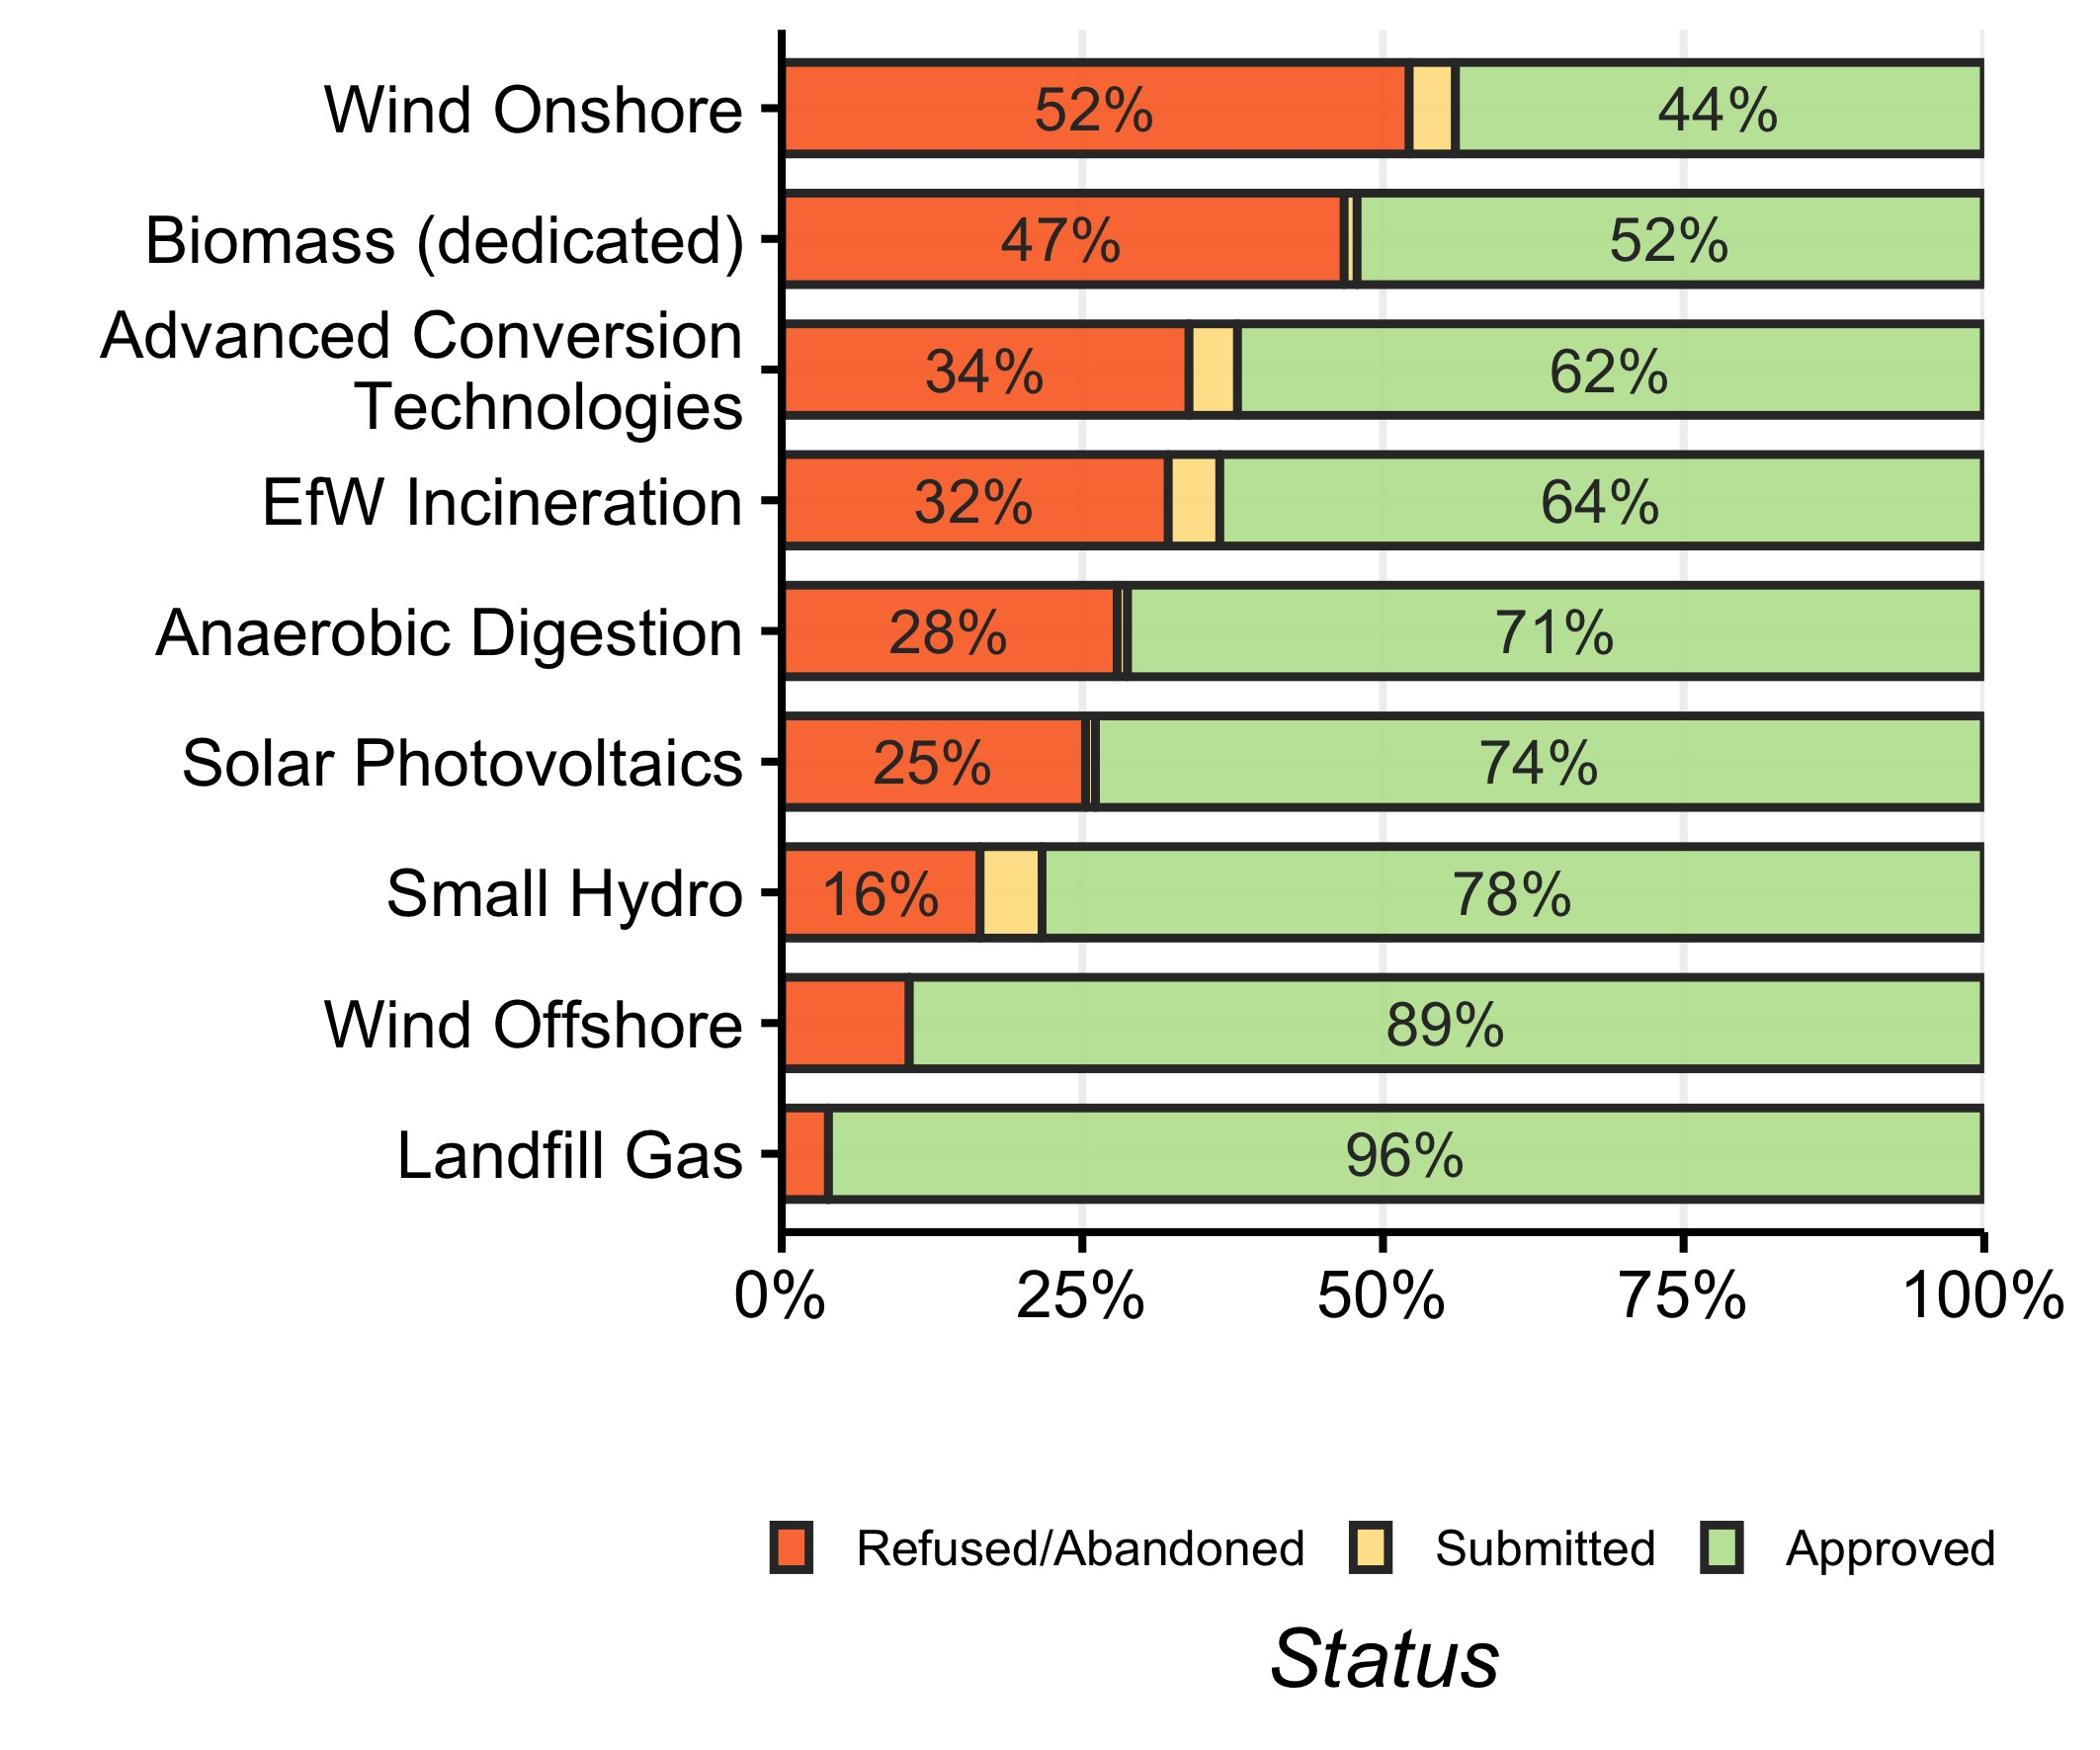
\includegraphics[width=0.5\linewidth]{figures/figure1} 

}

\caption{Acceptance rates of renewable energy projects
within the Great Britain between 1991 and 2017. The analysis only
considers technologies which have had more than 50 planning
applications.}\label{fig:acceptanceRates}
\end{figure}

Great Britain is not alone in encountering opposition to wind turbine
projects (Langer et al. \protect\hyperlink{ref-Langer2016}{2016}), but
is perhaps unique in how policy has been restructured to restrict it,
with recent changes in legislation severely impacting the further
development of onshore wind. Until June 2015, the planning decision for
projects greater than 50MW was controlled at a national level. This
provision was removed by the \emph{Energy Act 2016 cl 78} and
\emph{Infrastructure Planning (Onshore Wind Generating Stations) Order
2016}, which provided local authorities with the final say for all
onshore wind energy projects and only allows wind turbines to be
proposed in sites which have been identified within neighbourhood
development plans. These changes have effectively provided local
communities with a veto to block the development of wind turbines
(Cowell and Devine-Wright \protect\hyperlink{ref-Cowell2018}{2018}).

In addition to alterations in planning law, there have been changes to
the financial mechanisms used to support low-carbon energy in Great
Britain. Firstly, onshore wind projects were removed from the Renewable
Obligation scheme on 1st April 2016 under the \emph{Energy Act 2016} cl
79. Further to this, onshore wind projects are prevented from bidding in
the £557 million round of Contract for Differences auctions scheduled
for Spring 2019 (Smith \protect\hyperlink{ref-Smith2016}{2016}). Both
these financial changes have in effect restricted on the development of
onshore wind energy.

As a result of these planning and financial changes, there has been a
dramatic reduction in the development of onshore wind within Great
Britain. In June 2015, the month the changes in planning were
implemented, there were 133 planning applications for onshore wind, a
record high for a single month (DECC
\protect\hyperlink{ref-DECC2018}{2018}). In contrast, for the entire
year of 2017, there were only 52 planning applications made,
representing only 6\% of the 2015 total. This reduction in planning is
highlighted in Figure \ref{fig:numberApplications}.





\begin{figure}[h]

{\centering 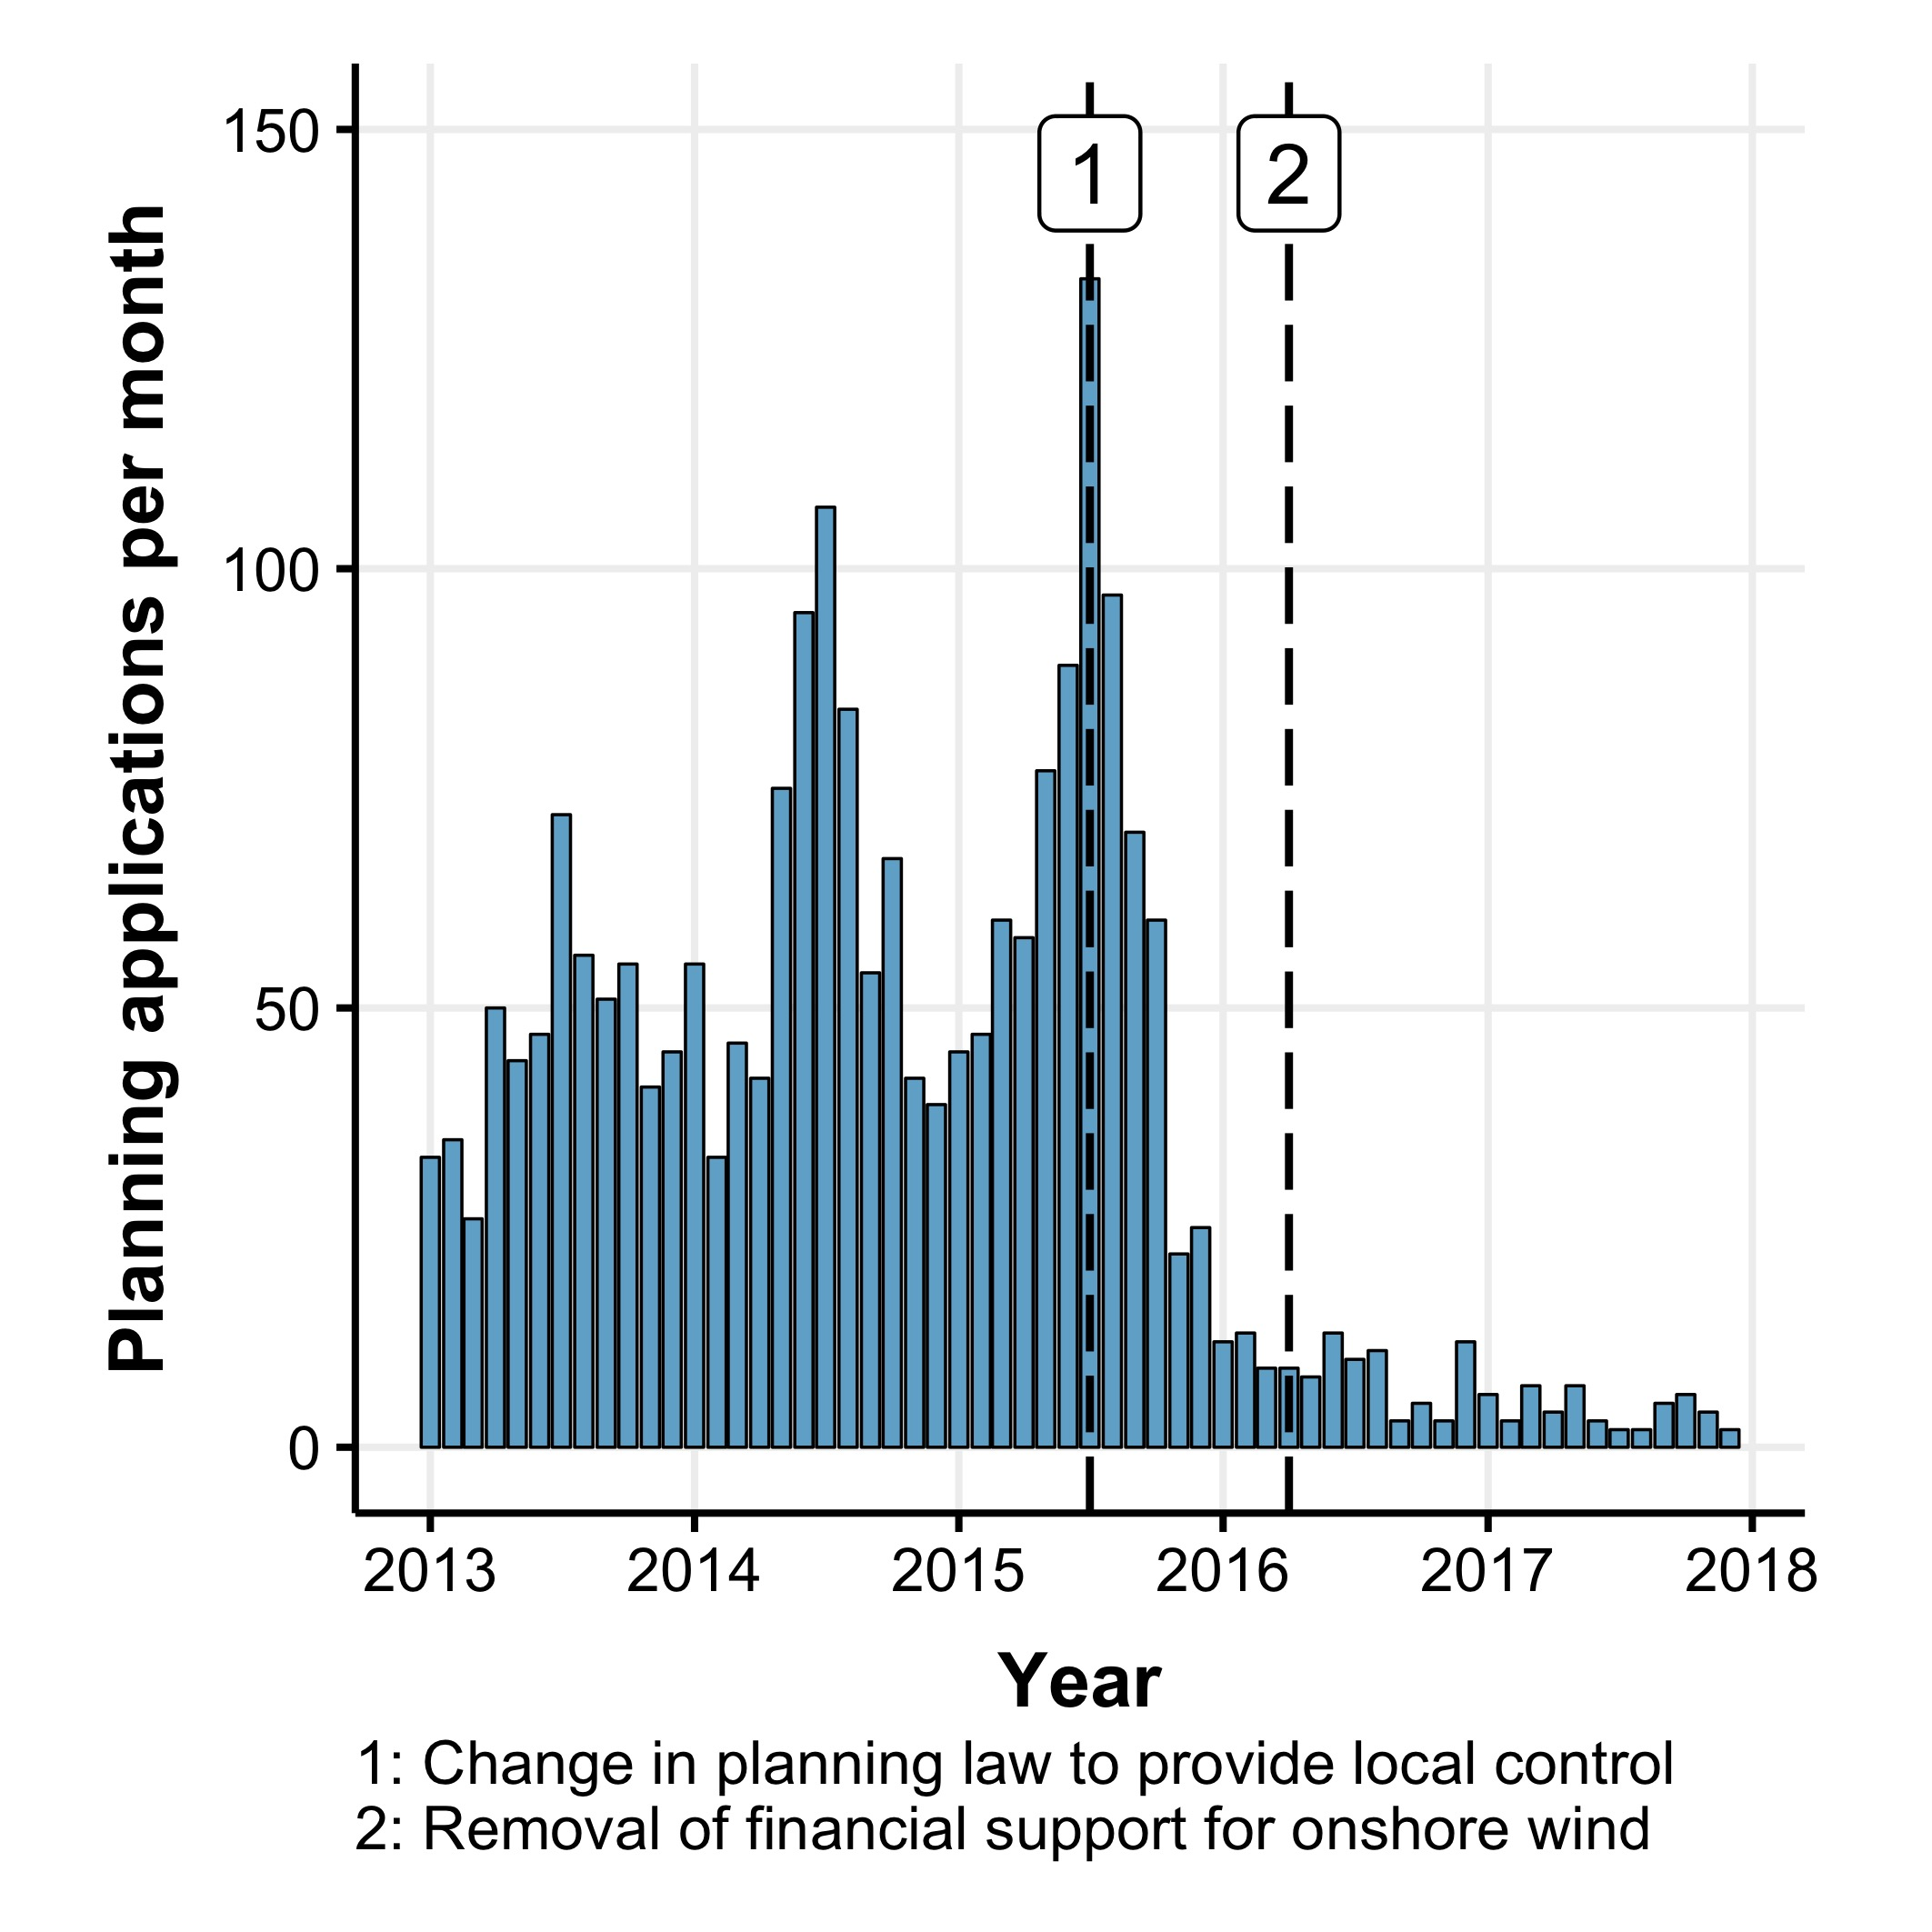
\includegraphics[width=0.5\linewidth]{figures/figure2} 

}

\caption{Number of turbine planning applications
submitted in the United Kingdom per month between January 2013 and
December 2017.}\label{fig:numberApplications}
\end{figure}

Whilst the predicted reduction of cost in onshore wind may soon overcome
the remaining financial barriers, the planning changes currently remain
as a major barrier to increased deployment. However, there have been
recent suggestions to soften the stance in planning to allow development
of projects in regions accepting of wind, most notably in Scotland and
Wales (\emph{Clean Growth Strategy/Outcomes of Bonn COP23, HC 596/597}).
In addition, the public approval of onshore wind in Great Britain
reached a record high of 76\% in April 2018 (Department for Business
Energy \& Industrial Strategy \protect\hyperlink{ref-DBIES2018}{2018}).
This therefore highlights the need to consider the influence of local
communities within the proposals of onshore wind projects and understand
characteristics which may be associated with project rejection.

There is an established precedent of using geospatial parameters to
assess the site suitability of onshore wind (Voivontas et al.
\protect\hyperlink{ref-Voivontas1998}{1998}; Baban and Parry
\protect\hyperlink{ref-Baban2001}{2001}). This paper seeks to understand
if existing geospatial modelling of onshore wind can account for the low
levels of acceptance of onshore wind in Great Britain (Figure
\ref{fig:acceptanceRates}) and then tests the extent to which existing
social and demographic parameters can be used to enhance acceptance rate
prediction for a site.

\hypertarget{background}{%
\section{Background}\label{background}}

The background covers three key sections of literature. Firstly, a
review of existing geospatial models is provided to understand how
suitable sites for onshore wind are determined. Issues relating to the
social acceptance of wind turbine are then presented to highlight the
broader social influences relating to onshore wind energy. Finally,
statistical techniques used to understand acceptance rates of wind
energy projects are reviewed.

\hypertarget{GIS}{%
\subsection{Geospatial modelling of onshore wind}\label{GIS}}

To assist in the development of onshore wind energy, many geospatial
methodologies have been produced to determine site suitability for wind
farms. Development primarily started in the late 1990s (Voivontas et al.
\protect\hyperlink{ref-Voivontas1998}{1998}; Baban and Parry
\protect\hyperlink{ref-Baban2001}{2001}), and established a structure
which has since been applied extensively internationally (Hansen
\protect\hyperlink{ref-Hansen2005}{2005}; Yue and Wang
\protect\hyperlink{ref-Yue2006}{2006}; Lee, Chen, and Kang
\protect\hyperlink{ref-Lee2009}{2009}; Janke
\protect\hyperlink{ref-Janke2010}{2010}; SQW Energy
\protect\hyperlink{ref-SQWEnergy2010}{2010}; Aydin, Kentel, and Duzgun
\protect\hyperlink{ref-Aydin2010}{2010}; Van Haaren and Fthenakis
\protect\hyperlink{ref-VanHaaren2011}{2011}; Sliz-Szkliniarz and Vogt
\protect\hyperlink{ref-Sliz-Szkliniarz2011}{2011}; Gass et al.
\protect\hyperlink{ref-Gass2013}{2013}; Neufville
\protect\hyperlink{ref-Neufville2013}{2013}; Miller and Li
\protect\hyperlink{ref-Miller2014}{2014}; Wang, M'Ikiugu, and Kinoshita
\protect\hyperlink{ref-Wang2014}{2014}; Watson and Hudson
\protect\hyperlink{ref-Watson2015}{2015}; Noorollahi, Yousefi, and
Mohammadi \protect\hyperlink{ref-Noorollahi2015}{2015}; Atici et al.
\protect\hyperlink{ref-Atici2015}{2015}; Baseer et al.
\protect\hyperlink{ref-Baseer2017}{2017}; Gigović et al.
\protect\hyperlink{ref-Gigovic2017}{2017}; Mentis et al.
\protect\hyperlink{ref-Mentis2017}{2017}; Manomaiphiboon et al.
\protect\hyperlink{ref-Manomaiphiboon2017}{2017}; Liu, Wang, and Zhu
\protect\hyperlink{ref-Liu2017}{2017}; Kazak, Hoof, and Szewranski
\protect\hyperlink{ref-Kazak2017}{2017}). These methodologies combine
geospatial modelling with Multi-criteria Decision Analysis (MCDA)
techniques, whereby various spatial attributes are combined into a
single scoring criteria to identify sites which are deemed suitable for
development (Malczewski \protect\hyperlink{ref-Malczewski2004}{2004}).
Ideal sites are typically identified as those which have good economic
viability, are not in areas where development is prohibited and have
minimal impact on local communities. Although the parameters vary for
studies, suitable sites for development will usually be determined as:
1) \emph{having high average wind speeds}; 2) \emph{not being close to
urban areas}; 3) \emph{not being in protected landscapes} (e.g.~National
Parks); 4) \emph{not close to airports} (to minimise radar
interference); 5) \emph{close to roads} (for site access) and 6)
\emph{close to power lines} (for grid connection).

Whilst models are typically based of an implicit assumption that
geospatial parameters can be used to determine suitable sites, there are
concerns that geospatial parameters in isolation are in themselves
insufficient to explain patterns of development of wind turbines (Horst
and Toke \protect\hyperlink{ref-VanderHorst2010}{2010}; Toke
\protect\hyperlink{ref-Toke2005}{2005}). In particular, it is argued
that modelling approaches are unable to fully capture the social
barriers surrounding the development of onshore wind energy (Langer et
al. \protect\hyperlink{ref-Langer2016}{2016}). This gap between
modelling and development can be highlighted by Figure
\ref{fig:acceptanceRatesWind}, which shows that despite widespread
interest in modelling the site suitability of onshore wind farms in the
UK, there has been an continuing decrease in the likelihood of wind
turbines receiving planning permission.

\begin{figure}[h]

{\centering 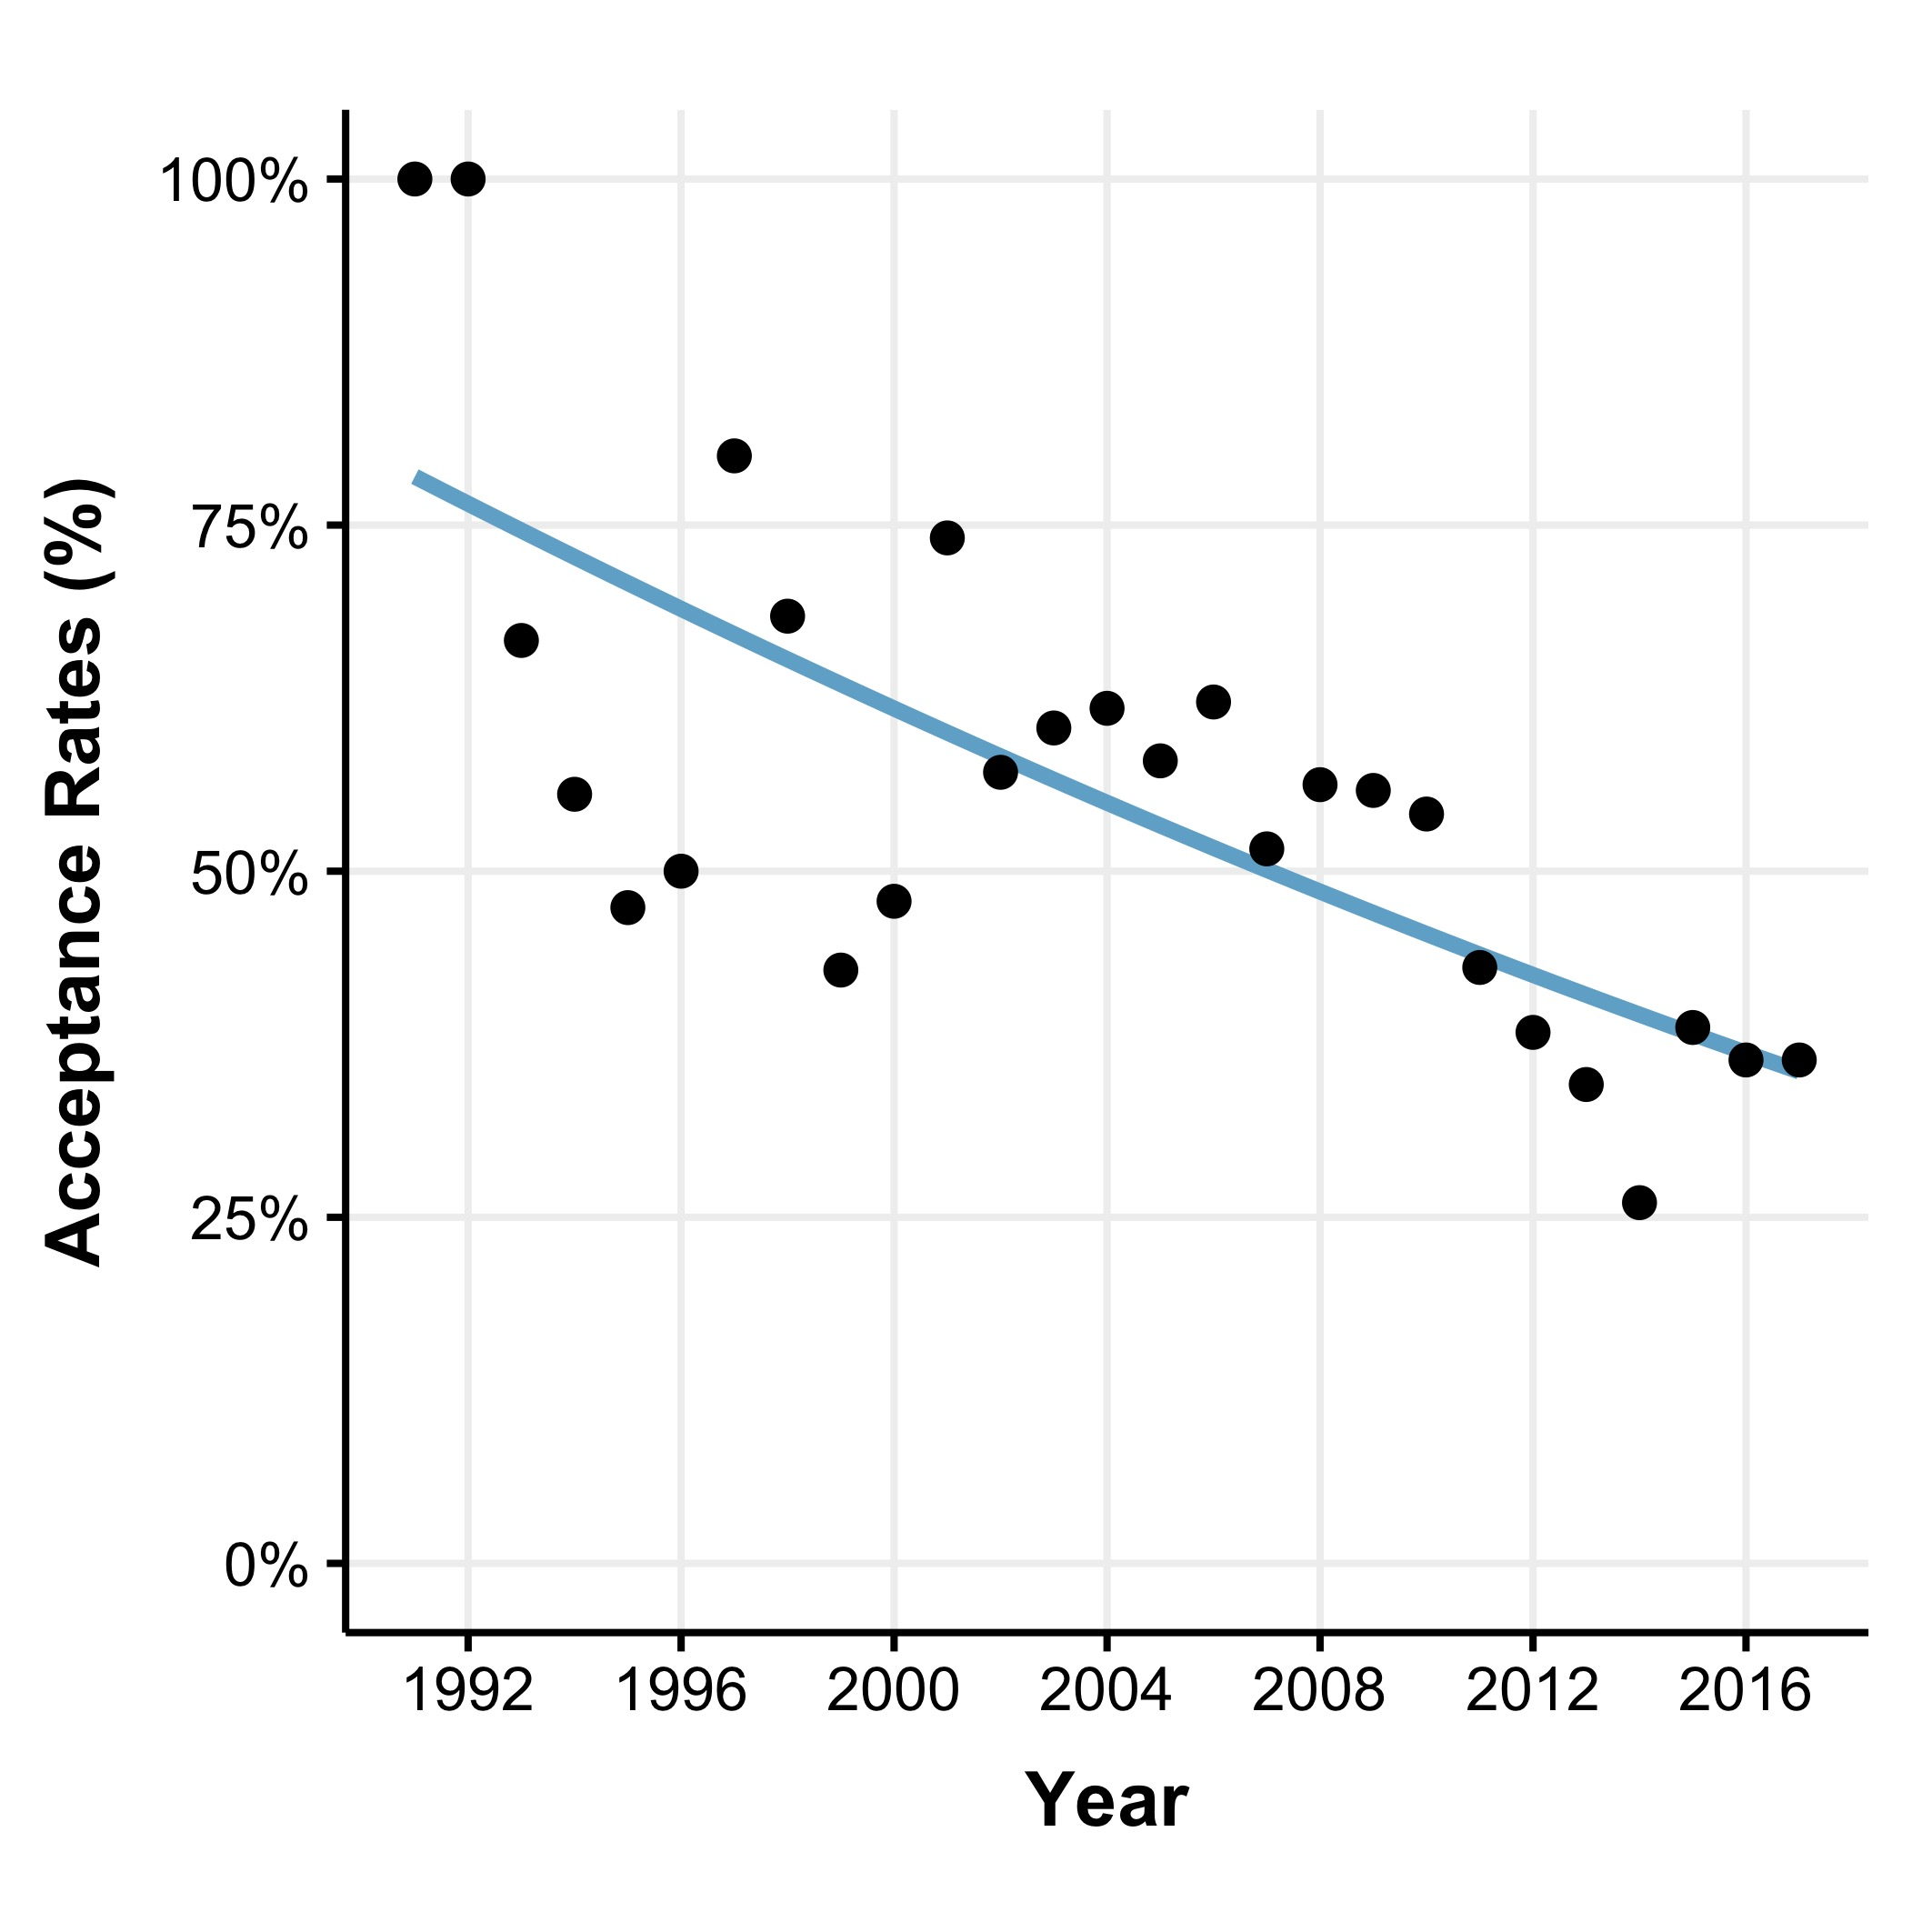
\includegraphics[width=0.5\linewidth]{figures/figure3} 

}

\caption{Annual average acceptance rate of wind turbine projects within Great Britain, 1990 to 2017. Line shows polynomial fitted relationship.}\label{fig:acceptanceRatesWind}
\end{figure}

Whilst some studies compare the resulting suitability maps with
locations of operational wind turbines (Watson and Hudson
\protect\hyperlink{ref-Watson2015}{2015}; Miller and Li
\protect\hyperlink{ref-Miller2014}{2014};; Gass et al.
\protect\hyperlink{ref-Gass2013}{2013}; Van Haaren and Fthenakis
\protect\hyperlink{ref-VanHaaren2011}{2011}; Aydin, Kentel, and Duzgun
\protect\hyperlink{ref-Aydin2010}{2010}), these were largely used only
as a form of discussion, and the information was not directly used to
develop or revise the models. This overlooks a valuable contribution
that existing sites could provide in understanding whether there are any
spatial development patterns which can be identified. In particular,
Watson (\protect\hyperlink{ref-Watson2015}{2015}) noted
``\emph{operational wind farms in South Central England were
predominantly located in areas suggested to be of lower suitability}'',
suggesting that the proposed model inaccurately assessed site
suitability in the region.

In situations where there is a large enough sample of similar historical
spatial decisions, an ``\emph{Inverse theory}'' approach can be applied
to determine subjective valuation of criteria by stakeholders (Cirucci
\protect\hyperlink{ref-Cirucci2014}{2014}). Compared to the traditional
``\emph{Forward theory}'' approach of geospatial modelling (Figure
\ref{fig:InverseGIS}a), an inverse approach assesses the existing
spatial distribution of projects to determine the most influential
parameters in determining site success (Figure \ref{fig:InverseGIS}b).
Such an approach has been used successfully within both public health
studies (Brody et al. \protect\hyperlink{ref-Brody2002}{2002}; Mohamed
et al. \protect\hyperlink{ref-Mohamed2004}{2004}; Yamada, Rogerson, and
Lee \protect\hyperlink{ref-Yamada2009}{2009}; Garcia-Ayllon
\protect\hyperlink{ref-Garcia-Ayllon2013}{2013}) and infrastructure
location decision-making (US EPA and Recovery
\protect\hyperlink{ref-USEPA2002}{2002}; Cirucci, Miller, and Blanford
\protect\hyperlink{ref-Cirucci2015}{2015}) to determine optimal sites
for development. However, there have been no examples identifed of this
approach being used within onshore wind energy modelling.

\begin{figure}[h]

{\centering 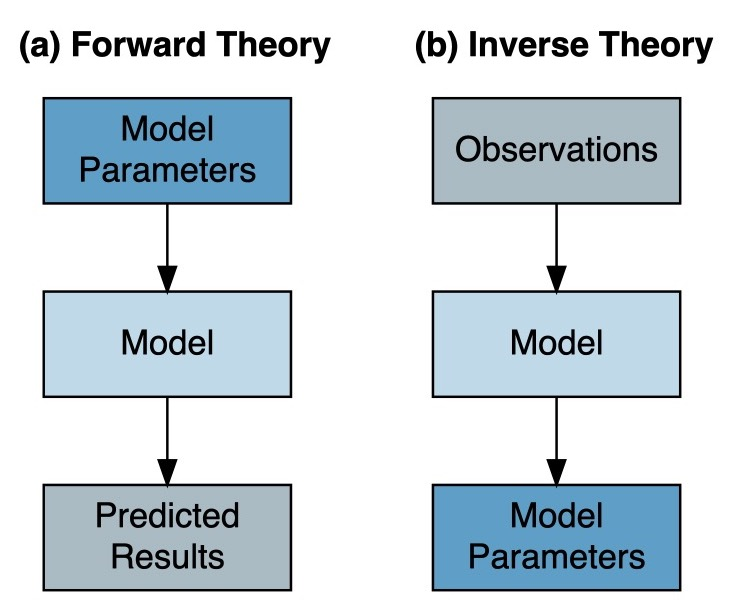
\includegraphics[width=0.5\linewidth]{figures/figure4} 

}

\caption{Comparison of Forward and Inverse GIS MCDA model structures}\label{fig:InverseGIS}
\end{figure}

\hypertarget{acceptance}{%
\subsection{Social acceptance of wind turbines}\label{acceptance}}

Traditional onshore wind GIS models focus on identfying sites which meet
technical and legislative criteria. However, there is a crucial
difference between what makes a site acceptable in a planning sense, and
what is acceptable to the local community. This has prompted research to
assess the factors which influence the public acceptance of onshore wind
turbines (Langer et al. \protect\hyperlink{ref-Langer2016}{2016}).
Although several definitions are provided (Upham, Oltra, and Boso
\protect\hyperlink{ref-Upham2015}{2015}, 107), the definition of social
acceptance adopted within this study is:

\begin{quote}
``a favourable or positive response (including attitude, intention,
behaviour and - where appropriate - use) relating to proposed or in situ
technology or social technical system by members of a given social unit
(country or region, community or town and household, organisation)''.
\end{quote}

Social acceptance parameters are summarised into three groups 1):
\emph{Physical and Environmental}; 2) \emph{Pyscho-social} and 3)
\emph{Social and Institutional} (Langer et al.
\protect\hyperlink{ref-Langer2016}{2016}). Stated-preference surveys are
frequently used to assess the views of individuals against wind energy
and identify factors which create positive or negative perceptions of
projects, with the key findings outlined below.

A concept consistently investigated within empirical research is the
\emph{``proximity hypothesis''}, which states that those living closest
to a wind farm will have the most negative perceptions of it
(Devine-Wright
\protect\hyperlink{ref-Devine-Wright2005}{2005}\protect\hyperlink{ref-Devine-Wright2005}{b};
Warren et al. \protect\hyperlink{ref-Warren2005}{2005}). However,
attempts to prove this hypothesis have largely proved unsuccessful, with
conflicting results. For example, evidence from Denmark suggests no link
between proximity of residential properties to the nearest turbine and
negative public perceptions, with suggestions that respondents living
closest (i.e.~within 500 metres) actually had more positive perceptions
in comparison with individuals living away from turbines (Krohn and
Damborg \protect\hyperlink{ref-Krohn1999}{1999}). This view was further
supported by a study in Cornwall, UK, which found that local communities
with visibility of the turbines were generally more supportive of wind
turbines (Eltham, Harrison, and Allen
\protect\hyperlink{ref-Eltham2008}{2008}). However, several studies have
reported the opposite relationship (Meyerhoff, Ohl, and Hartje
\protect\hyperlink{ref-Meyerhoff2010}{2010}; Ladenburg
\protect\hyperlink{ref-Ladenburg2008}{2008}), with the studies finding
that negative perceptions increased with proximity to wind energy
developments, althought these studies explored smaller sized turbines
along with different national contexts, and therefore may capture
different results.

Literature has also sought to understand the potential cumulative
effects that wind turbines have, as projects are frequently refused
planning in regions already containing wind turbines (Strachan and Lal
\protect\hyperlink{ref-Strachan2004}{2004}; Jones, Orr, and Eiser
\protect\hyperlink{ref-Jones2011}{2011}; Eltham, Harrison, and Allen
\protect\hyperlink{ref-Eltham2008}{2008}). However, there is limited
understanding of how neighbouring wind energy projects may alter the
likelihood of nearby wind turbine projects receiving planning, and
current research has focussed on smaller case studies (Jones, Orr, and
Eiser \protect\hyperlink{ref-Jones2011}{2011}).

It has also been highlighted within literature that psycho-social
factors have become crucial dimensions to explain how local communities
interact with, and react to, new wind farm developments (Langer et al.
\protect\hyperlink{ref-Langer2016}{2016}; Scherhaufer et al.
\protect\hyperlink{ref-Scherhaufer2017}{2017}). The effects of
socio-demographic variables on individuals' views of wind farms have
also been studied (Devine-Wright
\protect\hyperlink{ref-Devine-Wright2005}{2005}\protect\hyperlink{ref-Devine-Wright2005}{b};
Warren and McFadyen \protect\hyperlink{ref-Warren2010}{2010}), with 1)
\emph{age}; 2) \emph{gender}; 3) \emph{experience with wind farms} and
4) \emph{use of the land} found to be slightly correlated with the
attitudes towards wind power (Warren and McFadyen
\protect\hyperlink{ref-Warren2010}{2010}).

Empirical findings also suggest that political beliefs are correlated
with social acceptance of different low carbon technologies
(Devine-Wright \protect\hyperlink{ref-Devine-Wright2007}{2007}). The
shift towards anti-onshore wind was a key manifesto commitment of the
Conservative Party in the 2015 general election, and previous surveys
indicate that only 62\% of individuals who indicated support for the UK
Conservative Party were also supportive of new renewable energy
developments, compared to 86\% and 84\% for Labour and Liberal Democrats
respectively (Populus \protect\hyperlink{ref-Populus2005}{2005}).

Studies have highlighted that the interaction of developers with local
communities are also key indicators of positive planning approval
outcomes (Toke \protect\hyperlink{ref-Toke2005}{2005}; Devine-Wright
\protect\hyperlink{ref-Devine-Wright2005a}{2005}\protect\hyperlink{ref-Devine-Wright2005a}{a};
Wustenhagen, Wolsink, and Burer
\protect\hyperlink{ref-Wustenhagen2007}{2007}). People are generally
more supportive when projects seek greater consultation and community
interaction within their plans, compared to those which are fixed prior
to consultation with the local population.

Finally, the ownership structure of a project has been indicated to be a
significant influence on the level of public acceptance (Sonnberger and
Ruddat \protect\hyperlink{ref-Sonnberger2017}{2017}; Haggett and Toke
\protect\hyperlink{ref-Haggett2006}{2006}). Projects are generally seen
as more favourable when owned by local energy cooperatives rather than
by a large energy company or investor with no local connections and has
been suggested as a major factor explaining the differences in project
success between the United Kingdom and Germany (Toke, Breukers, and
Wolsink \protect\hyperlink{ref-Toke2008}{2008}).

\hypertarget{planning-acceptance-of-wind-energy-projects}{%
\subsection{Planning acceptance of wind energy
projects}\label{planning-acceptance-of-wind-energy-projects}}

Whilst studies have aimed to understand the social acceptance of onshore
wind turbines at an individual level, it is more beneficial to planners
and developers to understand how these influence the overall planning
acceptance of a wind energy project. There has been increased use of
quantitative analysis to understand the effect social and institutional
parameters have on the outcome of wind energy planning outcomes, with
four key studies being identified (Toke
\protect\hyperlink{ref-Toke2005}{2005}; Horst and Toke
\protect\hyperlink{ref-VanderHorst2010}{2010}; Rensburg, Kelley, and
Jeserich \protect\hyperlink{ref-VanRensburg20}{2015}; Roddis et al.
\protect\hyperlink{ref-Roddis2018}{2018}). Such approaches build upon
the understandings provided within the qualitative analysis explained
with Section \ref{acceptance}, but aim to identify key parameters and
their influence on the chance of a turbine receiving planning
permission.

A key determinant in the statistical power of the models is the number
of planning applications used within their models. The listed studies
used samples sizes of 51 (Toke \protect\hyperlink{ref-Toke2005}{2005}),
77 (Horst and Toke \protect\hyperlink{ref-VanderHorst2010}{2010}) 354
(Rensburg, Kelley, and Jeserich
\protect\hyperlink{ref-VanRensburg20}{2015}) and 1324 (Roddis et al.
\protect\hyperlink{ref-Roddis2018}{2018}) wind energy projects
respectively. These samples sizes influenced the suitability of the
modelling used: where a small sample size was used, the analysis used
univariate analysis to assess the influence of each parameter
individually, with logistic regression being used to assess each
independent variable individually (Toke
\protect\hyperlink{ref-Toke2005}{2005}; Horst and Toke
\protect\hyperlink{ref-VanderHorst2010}{2010}). Where larger sample
sizes are available multiple regression model approaches were used, with
probit (Rensburg, Kelley, and Jeserich
\protect\hyperlink{ref-VanRensburg20}{2015}) and logistic regression
(Roddis et al. \protect\hyperlink{ref-Roddis2018}{2018}) methods being
applied.

The studies explored the influence of social, demographic, poltical and
institutional parameters identified within the previous qualitative
analysis, although the scope of these parameters included varied between
studies. Toke (Toke \protect\hyperlink{ref-Toke2005}{2005}) assessed how
planning outcomes were influenced by the views of key actors within the
planning process of wind energy, including local councils, planning
authorities and landscape protection groups. Van der Horst and Toke
(\protect\hyperlink{ref-VanderHorst2010}{2010}) focussed on local
characteristics relating to education, health, demography, employment.
Van Rensburg et al.~(Rensburg, Kelley, and Jeserich
\protect\hyperlink{ref-VanRensburg20}{2015}) assessed project
technology, institutional processes and site endowment parameters.
Finally, Roddis et al.~(Roddis et al.
\protect\hyperlink{ref-Roddis2018}{2018}) developed a similar model as
previously developed by the authors (Harper et al.
\protect\hyperlink{ref-Harper2017}{2017}), using 26 parameters including
technical, aesthetic and local characteristics, but with a focus on
community acceptance of projects instead of planning approval.

Several key influential paremeters were identified across different
parameter groups. For socio-demographics, it was shown that planning
acceptance rates were closely associated with the high levels of
apprehension about such schemes amongst people living in the immediate
vicinity, highlighting the importance that social influences have on
planning acceptance (Toke \protect\hyperlink{ref-Toke2005}{2005}).
Several strong associations were identified for planning refusal,
including 1) \emph{voter turnout} and 2) \emph{years of potential life
lost} (a measure of premature mortality). It was also noted that wind
energy appears to generally be more likely to receive planning
permission in deprived areas, with developers ``\emph{keen to avoid
relatively privileged communities and target areas where people are
thought to less likely put up a fight}'' (Horst and Toke
\protect\hyperlink{ref-VanderHorst2010}{2010}, 220).

Van Rensburg et al.~(\protect\hyperlink{ref-VanRensburg20}{2015})
indicated that 1) \emph{proximity to Natura 2000 sites} (a protected
landscape under the European Union); 2) \emph{sites with high bird
sensitivity}; 3) \emph{hub height} and 4) \emph{project capacity} were
key indicators to project success. In addition, the study noted that
proximity of the nearest dwellings and wind speeds appeared
insignificant, which is counter to the view reported within many
geospatial models which aim to locate wind turbines distant to towns and
cities.

Roddis et al.~(Roddis et al. \protect\hyperlink{ref-Roddis2018}{2018})
reported 8 parameters as being significant in influencing the planning
acceptance of projects. These include the 1) \emph{proximity to National
Parks}; 2) \emph{Project Size} and 3) \emph{Social deprivation}.
Interestingly, the study reports contrasting results to previous
research (Horst and Toke \protect\hyperlink{ref-VanderHorst2010}{2010}),
with it being reported that areas of low deprivation appeared more
likely to be accepting of onshore wind energy projects.

The studies by Van Rensburg et
al.~(\protect\hyperlink{ref-VanRensburg20}{2015}) and Roddis et
al.~(\protect\hyperlink{ref-Roddis2018}{2018}) attempted to produce an
overall statistical model to predict the likelihood of a wind turbine
receiving planning acceptance. Of the variables included within these
models provided an adjusted R\textsuperscript{2} value of 0.31 and 0.26
respectively.

\hypertarget{developing-integrated-site-suitability-assessment-models}{%
\subsection{Developing integrated site suitability assessment
models}\label{developing-integrated-site-suitability-assessment-models}}

Given the prevalence of GIS modelling in determining suitable sites, and
the relatively high level of rejection of projects within the UK, it is
argued that there a need to understand how geospatial parameters
influence the acceptance rates of projects. The studies referenced in
Section \ref{GIS} have suggested a relationship between local
demographic and social attributes and wind turbine planning acceptance
rates, yet none attempted to integrate these findings into their site
suitability tools beyond the use of proximity buffers around urban
areas. This omission means that social dimensions have generally not
been factored in to assessments of the suitability of sites for onshore
wind development.

Responding to calls to combine qualitative and quantitative research
(Langer et al. \protect\hyperlink{ref-Langer2016}{2016}, 256), this
paper presents analysis which assesses parameters that influence wind
turbine planning outcomes, utilising a range of physical, geographical,
demographic and political parameters. Building upon the existing
quantitative studies (Toke \protect\hyperlink{ref-Toke2005}{2005}; Horst
and Toke \protect\hyperlink{ref-VanderHorst2010}{2010}; Rensburg,
Kelley, and Jeserich \protect\hyperlink{ref-VanRensburg20}{2015}; Roddis
et al. \protect\hyperlink{ref-Roddis2018}{2018}), the work reported
extends current knowledge through the use of a larger number of site
consent applications (n = 1,721) and a broader range of geospatial
parameters than has previously been the case.

\hypertarget{material-and-methods}{%
\section{Material and methods}\label{material-and-methods}}

The overall methodology is highlighted in Figure \ref{fig:Methodology},
with a detailed explanation provided in the following subsections. This
approach expands upon the methodology previously developed by the
authors (Harper et al. \protect\hyperlink{ref-Harper2017}{2017}; Harper
\protect\hyperlink{ref-Harper2018}{2018}). The analysis and report was
written using the R programming language (R Core Team
\protect\hyperlink{ref-R-base}{2018}) and R Markdown (Allaire et al.
\protect\hyperlink{ref-R-rmarkdown}{2018}), with the full statistical
analysis and turbine dataset provided with the supporting files to allow
for the results of a the analysis to be reproduced.

\begin{figure}[h]

{\centering 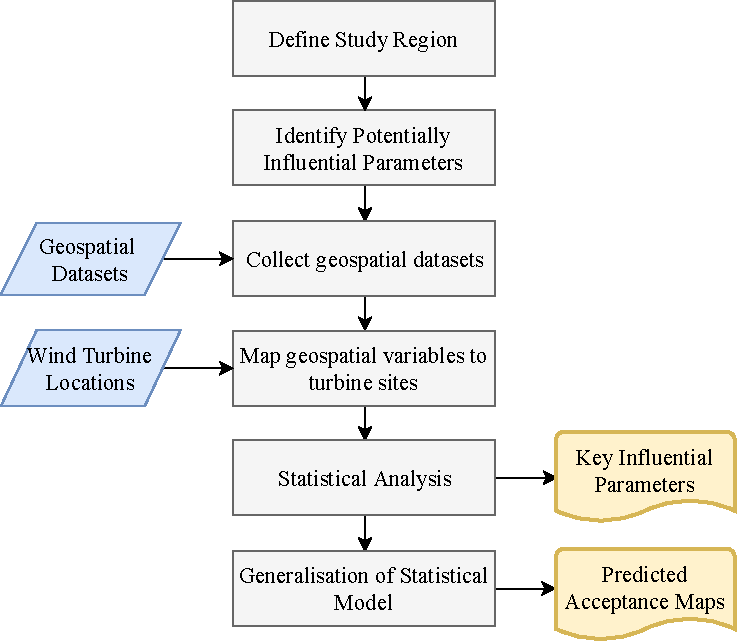
\includegraphics[width=0.75\linewidth]{../_figures/Flowchart/ResearchApproach} 

}

\caption{Research methodology to analyse patterns in onshore wind acceptance rates.}\label{fig:Methodology}
\end{figure}

\hypertarget{study-scope}{%
\subsection{Study scope}\label{study-scope}}

The study was conducted across Great Britain (England, Scotland \&
Wales). These regions were chosen due to the broadly similar
categorisation of land types, nature designation, data availability and
legislation across these regions (HM Government
\protect\hyperlink{ref-HMGovernment2014}{2014}). The Shetland Islands
were excluded from the analysis as their geographic isolation and
distance from mainland Britain created issues in generalising the model
results.

\hypertarget{wind-turbines-dataset}{%
\subsubsection{Wind turbines dataset}\label{wind-turbines-dataset}}

Information for turbine planning applications was collected through the
Renewable Energy Planning Database (REPD) (DECC
\protect\hyperlink{ref-DECC2018}{2018}). Although planning applications
detail are available until March 2018, projects were only considered up
until December 2015; the time at which the recent financial and planning
changes were made. Detailed information for each planning application
includes 1) \emph{location}; 2) \emph{year of application}; 3)
\emph{number of turbines}; 4) \emph{turbine capacity} and 5)
\emph{planning decision}.

The database includes detailed planning information with the planning
status. To simplify the use within the statistical modelling, this
status was summarised into a dichotomous variable with the variables: 1)
\emph{Approved} (Application Granted/Under Construction/Appeal
Granted/Operational/Decommission) and 2) \emph{Refused/Abandoned}
(Application Refused/Appeal Withdrawn/Abandoned). The spatial
distribution of these two groups of sites is shown in Figure
\ref{fig:StudyExtent}.

\begin{figure}[h]

{\centering 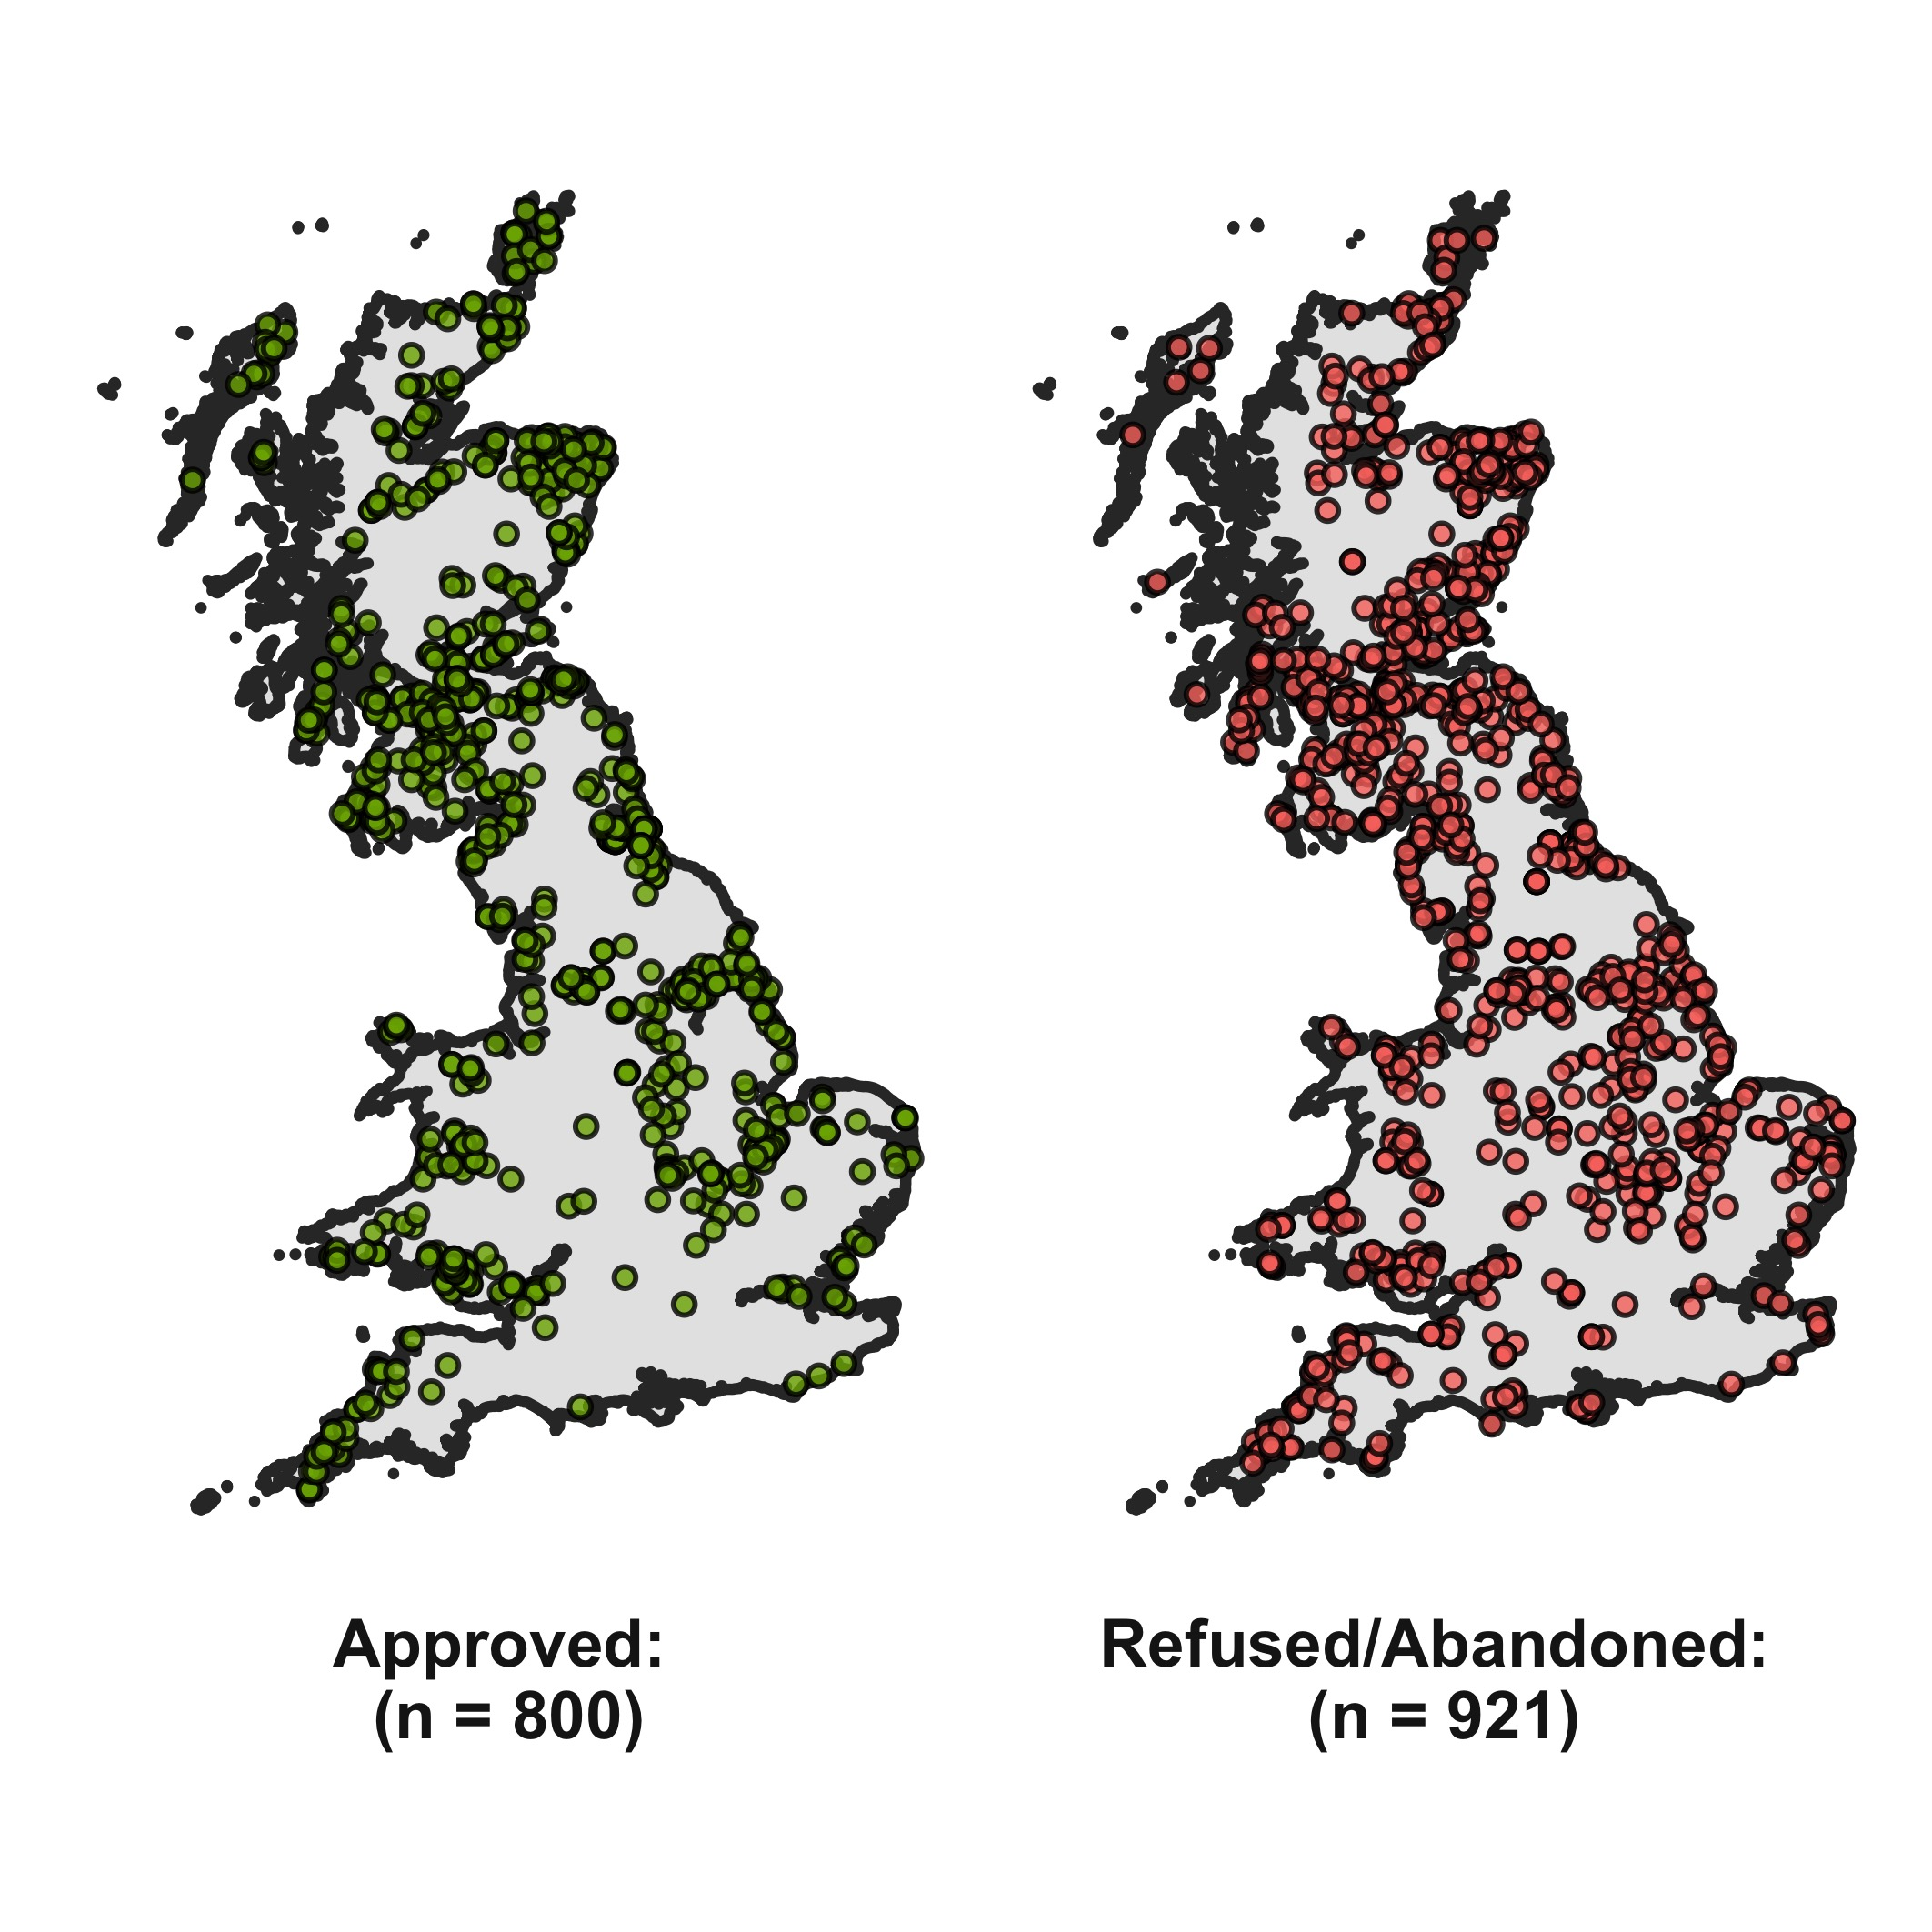
\includegraphics[width=0.5\linewidth]{figures/figure6} 

}

\caption{Location of onshore wind energy planning applications used within the study. Location data extracted from the Renewable Energy Planning Database (REPD) [DECC, 2018]}\label{fig:StudyExtent}
\end{figure}

\hypertarget{model-layers-data}{%
\subsubsection{Model layers data}\label{model-layers-data}}

Building upon the literature review in Section \ref{background}, data
sources were identified for physical, environmental and social
parameters at each turbine location which had been indicated to
influence wind turbine planning applications. A summary of the variables
is provided in Table \ref{tab:SummaryTable} and discussed below, with a
full details provided within the Technical Appendix A. Of the most
comparable work (Roddis et al.
\protect\hyperlink{ref-Roddis2018}{2018}), this study used a total of 30
parameters, 11 of which were common to both studies. These layers were
categorised as follows:

\begin{table}[t]

\caption{\label{tab:SummaryTable}Parameters considered within model}
\centering
\begin{threeparttable}
\begin{tabular}{ll}
\toprule
Category & Variable\\
\midrule
Turbine & Wind Turbine Planning Data\\
 & Turbine Capacity\\
 & Number of Turbines\\
 & Year\\
 & Country\\
Resource & Wind Speed\\
Features & Airports\\
 & Roads\textsuperscript{a}\\
 & Railways\\
 & Urban Areas\\
 & HV Powerlines\textsuperscript{b}\\
 & Military Sites\\
Landscape & Areas of Outstanding Natural Beauty\\
 & National Parks\\
 & Heritage Coast\\
Nature & Special Protection Areas\\
 & National Nature Reserve\\
 & Sites of Special Scientific Interest\\
 & Special Areas of Conservation\\
Geographic & Elevation\\
 & Slope\\
Census & Level of Qualification\textsuperscript{c}\\
 & Age\\
 & Social Grade\textsuperscript{d}\\
 & Tenure\\
Political & Conservatives\\
 & Labour\\
 & Liberal Democrat\\
Proximity & Nearest Turbine (Operational)\\
 & Nearest Turbine (Rejected)\\
\bottomrule
\end{tabular}
\begin{tablenotes}
\item[a] Roads are broken into four main categories: Motorways, A Roads, B Roads and Minor Roads
\item[b] High Voltage network from 132 kV to 400 kV
\item[c] L4 represents degree level or above
\item[d] AB represents Higher and intermediate managerial, administrative, professional occupation
\end{tablenotes}
\end{threeparttable}
\end{table}

\begin{itemize}
\tightlist
\item
  \textbf{Wind Resource}: wind speeds were taken from the Numerical
  Objective Analysis of Boundary Layer (NOABL) wind speed database. This
  provides estimated annualised wind speed at 45m elevation at a
  resolution of 1km grid (DTI \protect\hyperlink{ref-DTI2001}{2001}).
\item
  \textbf{Landscape Features}: Physical features including roads,
  railways and urban areas were collected from OS Strategi (Ordnance
  Survey \protect\hyperlink{ref-Survey2016}{2016}). The electricity
  transmission network, military sites and airport locations (civil and
  military) were extracted from Open Street Maps (OSM) (OSM
  \protect\hyperlink{ref-Overpass2016}{2016}).
\item
  \textbf{Landscape and Nature}: Landscape and nature designations were
  collected for regions within Great Britain (Pope
  \protect\hyperlink{ref-Pope2017}{2017}).
\item
  \textbf{Geographic}: Site elevation data was collected at a 25m
  resolution (European Commission
  \protect\hyperlink{ref-Commission2015}{2015}). This was used to
  calculate the gradient using the Fleming and Hoffer algorithm (Fleming
  and Hoffer \protect\hyperlink{ref-Fleming1979}{1979}).
\item
  \textbf{Demographic}: Census data was collected at the Lower Super
  Output Area (LSOA) and Data Zone (Scotland) for each turbine location.
  LSOAs and Data Zones represent regions with a population between 1000
  and 3000 people (Office for National Statistics
  \protect\hyperlink{ref-OfficeforNationalStatistics}{2016}).\\
\item
  \textbf{Political}: Political data was collected at the local
  authority level for the four largest parties in Great Britain: 1)
  \emph{Conservatives}; 2) \emph{Labour}, 3) \emph{Liberal Democrat} and
  4) \emph{Scottish National Party (SNP)} between 1990 and 2016. These
  parties held a sum of 95\% of council seats within Great Britain as of
  2016.
\item
  \textbf{Cumulative local turbines}: the nearest wind turbine to the
  project was calculated using the location and year of planning
  application for each turbine.
\end{itemize}

Guidance states that that the location of wind turbines should consider
sensitive birds and migratory flight paths (Gove et al.
\protect\hyperlink{ref-Gove2013}{2013}). Although maps are available for
parts of the study region (Bright et al.
\protect\hyperlink{ref-Bright2006}{2006}), it was not possible to
collect bird sensitivity maps for the whole study region. It was
therefore decided to not include this data within the statistical model.
However, as proposed projects are required to conduct an Environmental
Impact Assessment, sites which are found to impact birds will often be
abandoned before planning permission is sought, and therefore it is
argued that such impacts should not influence the planning outcome.

\hypertarget{data-transformations}{%
\subsection{Data transformations}\label{data-transformations}}

The data sources came as raster and vector spatial features, which were
aggregated at each of the turbine locations as follows:

\begin{itemize}
\tightlist
\item
  \textbf{Points, lines and polygons}: A spatial join was completed to
  find the distance to the nearest feature for each turbine. For polygon
  based data source, a value of 0km denotes the turbine is within the
  feature. Left censoring was used to limit the maximum distance of
  geospatial relationships to 30km, which is recommended within
  literature as the maximum typical distance at which the visual
  interference of wind turbines should be considered (SNH
  \protect\hyperlink{ref-SNH2009}{2009}).
\item
  \textbf{Tabular}: corresponding political and census boundaries were
  used to map the tabular data, and turbines assigned the value of the
  region. In addition, political data was filtered to the year of the
  planning application to determine the political balance at the time of
  planning.
\item
  \textbf{Raster}: The raster value at the site location was extracted.
\end{itemize}

In comparison to previous research (Rensburg, Kelley, and Jeserich
\protect\hyperlink{ref-VanRensburg20}{2015}), no transformations were
made to the standardise the dataset. Transformation provides no direct
benefit to the model other than to allow a direct comparison to be made
between the influence of parameters. In addition, transformed model
parameters create additional complications in the generalising of model
results as the model layers must be transformed to the adjusted layers
(Harrell \protect\hyperlink{ref-Harrell2001}{2001}, 123).

\hypertarget{statistical-modelling}{%
\subsection{Statistical modelling}\label{statistical-modelling}}

A multiple logistic regression analysis was conducted to model the
factors associated with a positive planning outcome of wind turbine
applications using the predictor variables listed in Table
\ref{tab:SummaryTable}. This model extends the approaches developed
within previous studies (Toke \protect\hyperlink{ref-Toke2005}{2005};
Rensburg, Kelley, and Jeserich
\protect\hyperlink{ref-VanRensburg20}{2015}; Roddis et al.
\protect\hyperlink{ref-Roddis2018}{2018}). A hierarchical approach was
applied to the model whereby parameters are added to the model
sequentially based on the presumed importance of parameters. These were
selected as follows:

\begin{enumerate}
\def\labelenumi{\arabic{enumi}.}
\tightlist
\item
  \textbf{Aspatial site attributes}: variables including \emph{Number of
  Turbines} and \emph{Installed Capacity}.
\item
  \textbf{Economic considerations}: parameters which influence the cost
  effectiveness of the site, including \emph{Wind Speed} and
  \emph{Proximity to the National Grid}.
\item
  \textbf{Temporal}: the year in which the planning application was made
  to account for potential policy changes.
\item
  \textbf{Proximity to features}: proximity to geographic features,
  Landscape and Nature Designations
\item
  \textbf{Social attributes}: Demographic attributes for the area of the
  wind energy project
\item
  \textbf{Political attributes}: the political composition of the local
  authority at the time of the planning application.
\item
  \textbf{Spatial proximity to other turbines}: the proximity to the
  nearest wind energy project.
\end{enumerate}

For each additional set of parameters added to the model, diagnostic
checks were made to ensure that the assumptions of logistic regression
were maintained. Each parameter was checked for linearity of the logit
for independent variables, absence of multicollinearity and independence
of variables (Harrell \protect\hyperlink{ref-Harrell2001}{2001}). Any
parameters which violated these conditions were removed from the model.
The overall fit of the model was assessed using Pearson chi-squared,
Psuedo R\textsuperscript{2} values and the residual deviance. Internal
validation was used to assess the predictive accuracy of the model, with
a random sample of 5\% fold size randomly selected and iterated 200
times. Once all parameters had been included within the model, a
parsimonious model was produced to remove non-influential parameters,
with the Akaike Information Criterion (AIC) used to determine the best
fitting model. The full statistical analysis is provided as an
additional appendix.

Regional differences in parameter effects between England, Scotland and
Wales were hypothesised due to differing population densities (England:
413/km\textsuperscript{2}, Wales: 149/km\textsuperscript{2}, Scotland:
68/km\textsuperscript{2}) (ONS \protect\hyperlink{ref-ONS2013}{2013}) as
well as differing institutional support, with Scotland in particular
placing a greater emphasis on the development of onshore wind (DECC
\protect\hyperlink{ref-DECC2018}{2018}). Where significant variation is
expected within subgroups, split data models are recommended, whereby
the dataset is segmented into groups based on model variables, and
regression models are fitted to each subgroup (Stoltzfus
\protect\hyperlink{ref-Stoltzfus2011}{2011}). Whilst these differences
can be explored using a dummy variable, such an approach only captures
the level effect and not the slope effect, and therefore only allows for
limited variability between the subgroups. The work reported here
therefore created separate logistic regression models for each country
(England, Scotland, Wales). The parameters used to construct these
models used two approaches. Firstly, the parameters from the
parsimonious model were used across all three models (``\emph{Global
Parameter}''). Secondly, the parameters were independently iterated
within each of the three group models to identify the best-fitting set
for each country (``\emph{Optimised Parameters}'').

\hypertarget{generalisation}{%
\subsection{Generalisation}\label{generalisation}}

A model which can predict site suitability for existing sites does not
contribute to the assessment of future sites. Thus, in order to
generalise the model results to all areas of Great Britain and therefore
allow the model-based assessment of potential suitability, a spatial
regression model was produced to generalise the results to all areas.
This used the three-country parsimonious regression models to predict
sites nationally at a 500m grid resolution. This model contained 13
variables, two of which were non-spatial parameters: 1) \emph{Turbine
Capacity} and 2) \emph{Year}. To include these within the prediction,
fixed values were assumed, and predictions made for the year 2017 with a
turbine size of 2MW (the average model size for the given year (DECC
\protect\hyperlink{ref-DECC2018}{2018})).

\hypertarget{results}{%
\section{Results}\label{results}}

The overall results for each stage of the hierarchical model are
presented in Table \ref{tab:LogisticModelComparison}. It can be seen
that there is a improvement of the Nagelkirke R\textsuperscript{2}
values across the results from 0.014 (Model 1) to 0.206 (Model 7), and
similarly the predictive accuracy of the model improves as more
parameters are included. The final model (Model 7) reports a
Hosmer-Lemeshow p-value of 0.032, which validates the null hypothesis
for this model.

\begin{table}[!h]

\caption{\label{tab:LogisticModelComparison}A summary of the hierarchical logistic regression models}
\centering
\resizebox{\linewidth}{!}{
\begin{tabular}{llllllll}
\toprule
  & Model 1 & Model 2 & Model 3 & Model 4 & Model 5 & Model 6 & Model 7\\
\midrule
Observations & 1715 & 1715 & 1715 & 1715 & 1715 & 1715 & 1715\\
Parameters & 3 & 5 & 6 & 22 & 25 & 28 & 31\\
Deviance & 2351 & 2346 & 2248 & 2164 & 2131 & 2127 & 2082\\
R.n & 0.014 & 0.018 & 0.091 & 0.151 & 0.173 & 0.176 & 0.206\\
Chi Square & 19 & 24 & 121 & 205 & 238 & 242 & 287\\
Degrees of Freedom & 2 & 4 & 5 & 21 & 24 & 27 & 30\\
p & 9e-05 & 1e-04 & 0.000 & 0.000 & 0.000 & 0.000 & 0.000\\
Residual Deviance & 1712 & 1710 & 1709 & 1693 & 1690 & 1687 & 1684\\
AIC & 2357 & 2356 & 2260 & 2208 & 2181 & 2183 & 2144\\
Accuracy & 52.7\% & 53.5\% & 61.7\% & 64.3\% & 64.2\% & 64.5\% & 65.3\%\\
\bottomrule
\end{tabular}}
\end{table}

Table \ref{tab:LogisticResults} provides the results from the final
hierarchical regression model (Model 7). Statistically significant
positive trends (e.g.~increase in the parameter increases success rates)
were observed for 1) \emph{Turbine Capacity}; 2) \emph{Distance to Urban
Regions}; 3) \emph{Distance to Areas of Outstanding Natural Beauty
(AONB)} 4) \emph{Distance to National Parks} and 5) \emph{Distance to
Nearest Turbine (Rejected)}. Negative associations were found for 1)
\emph{Year}; 2) \emph{Distance to Ramsar sites}; 3) \emph{Distance to
Natura 2000 sites}; 4) \emph{Qualifications L4 (University degree or
above)}; 5) \emph{Mean Age} and 6) \emph{Nearest Turbine (Operational)}.

The total number of parameters retained in the parsimonious model was
reduced from 30 to 15. This resulted in a marginal penalty in
performance of the model, with the R\textsuperscript{2} values reducing
from 0.2 to 0.193. The odds ratios (OR) for these remaining parameters
are shown for each parameter in Figure \ref{fig:oddsPars}, whereby an OR
equal to 1 means the parameter does not affect odds of the planning
outcome, OR greater than 1 indicates the parameters positively influence
planning acceptance, OR less than 1 represents a negative parameter
influence.

\begin{table}[!h]

\caption{\label{tab:LogisticResults}Odds Table for Logistic Regression Parameters}
\centering
\resizebox{\linewidth}{!}{
\begin{tabular}{lrrrrlrrr}
\toprule
Variable & Estimate & Std. Error & z value & Pr & Sig. & Odds Ratio & OR 
 2.5\% CI & OR 
 97.5\% CI\\
\midrule
Number of Turbines & 0.002 & 0.006 & 0.406 & 0.685 &  & 1.002 & 0.991 & 1.014\\
Turbine Capacity MW & 0.371 & 0.068 & 5.496 & 0.000 & *** & 1.450 & 1.271 & 1.657\\
Wind Speed & -0.091 & 0.063 & -1.448 & 0.148 &  & 0.913 & 0.807 & 1.033\\
Distance to HV Powerlines & 0.002 & 0.009 & 0.244 & 0.807 &  & 1.002 & 0.985 & 1.021\\
Year & -0.119 & 0.014 & -8.517 & 0.000 & *** & 0.888 & 0.863 & 0.912\\
Distance to Airports & 0.008 & 0.004 & 2.067 & 0.039 & * & 1.008 & 1.000 & 1.015\\
Distance to A Roads & 0.003 & 0.013 & 0.247 & 0.805 &  & 1.003 & 0.979 & 1.028\\
Distance to B Roads & -0.033 & 0.019 & -1.717 & 0.086 & . & 0.968 & 0.932 & 1.005\\
Distance to Minor Roads & 0.050 & 0.071 & 0.702 & 0.482 &  & 1.051 & 0.915 & 1.207\\
Distance to Motorways & 0.000 & 0.007 & 0.014 & 0.989 &  & 1.000 & 0.987 & 1.014\\
Distance to Railways & 0.013 & 0.009 & 1.431 & 0.152 &  & 1.013 & 0.995 & 1.031\\
Distance to  Urban Region & 0.169 & 0.065 & 2.585 & 0.010 & ** & 1.184 & 1.042 & 1.347\\
Distance to AONB & 0.017 & 0.006 & 2.807 & 0.005 & ** & 1.017 & 1.005 & 1.029\\
Distance to National Park & 0.030 & 0.007 & 4.506 & 0.000 & *** & 1.030 & 1.017 & 1.044\\
Distance to Heritage Coast & -0.010 & 0.009 & -1.183 & 0.237 &  & 0.990 & 0.973 & 1.007\\
Distance to NNR & -0.004 & 0.007 & -0.564 & 0.573 &  & 0.996 & 0.982 & 1.010\\
Distance to Ramsar & 0.014 & 0.007 & 2.146 & 0.032 & * & 1.015 & 1.001 & 1.028\\
Distance to SACS & 0.004 & 0.010 & 0.438 & 0.661 &  & 1.004 & 0.985 & 1.023\\
Distance to Natura 2000 & -0.019 & 0.008 & -2.306 & 0.021 & * & 0.981 & 0.965 & 0.997\\
Distance to SSSI & 0.040 & 0.025 & 1.601 & 0.109 &  & 1.041 & 0.991 & 1.094\\
Distance to Military Sites & 0.001 & 0.008 & 0.084 & 0.933 &  & 1.001 & 0.985 & 1.016\\
Qualifications, L4 & -0.032 & 0.007 & -4.596 & 0.000 & *** & 0.968 & 0.955 & 0.981\\
Mean Age & -0.041 & 0.017 & -2.367 & 0.018 & * & 0.960 & 0.928 & 0.993\\
Home Ownership & 0.000 & 0.000 & 0.542 & 0.588 &  & 1.000 & 0.999 & 1.001\\
Political, Conservative Share & -0.001 & 0.003 & -0.305 & 0.760 &  & 0.999 & 0.992 & 1.006\\
Political, Labour Share & 0.005 & 0.004 & 1.279 & 0.201 &  & 1.005 & 0.997 & 1.013\\
Political, Liberal Democrat & 0.003 & 0.005 & 0.694 & 0.488 &  & 1.003 & 0.994 & 1.013\\
Nearest Turbine (Operational) & -0.017 & 0.004 & -4.238 & 0.000 & *** & 0.983 & 0.975 & 0.991\\
Nearest Turbine (Rejected) & 0.021 & 0.003 & 6.339 & 0.000 & *** & 1.021 & 1.015 & 1.028\\
Distance to  Large Urban Areas & -0.004 & 0.013 & -0.316 & 0.752 &  & 0.996 & 0.971 & 1.022\\
\bottomrule
\multicolumn{9}{l}{\textit{Signif. codes: } 0 '***' 0.001 '**' 0.01 '*' 0.05 '.' 0.1 ' ' 1}\\
\end{tabular}}
\end{table}

\begin{figure}[h]

{\centering 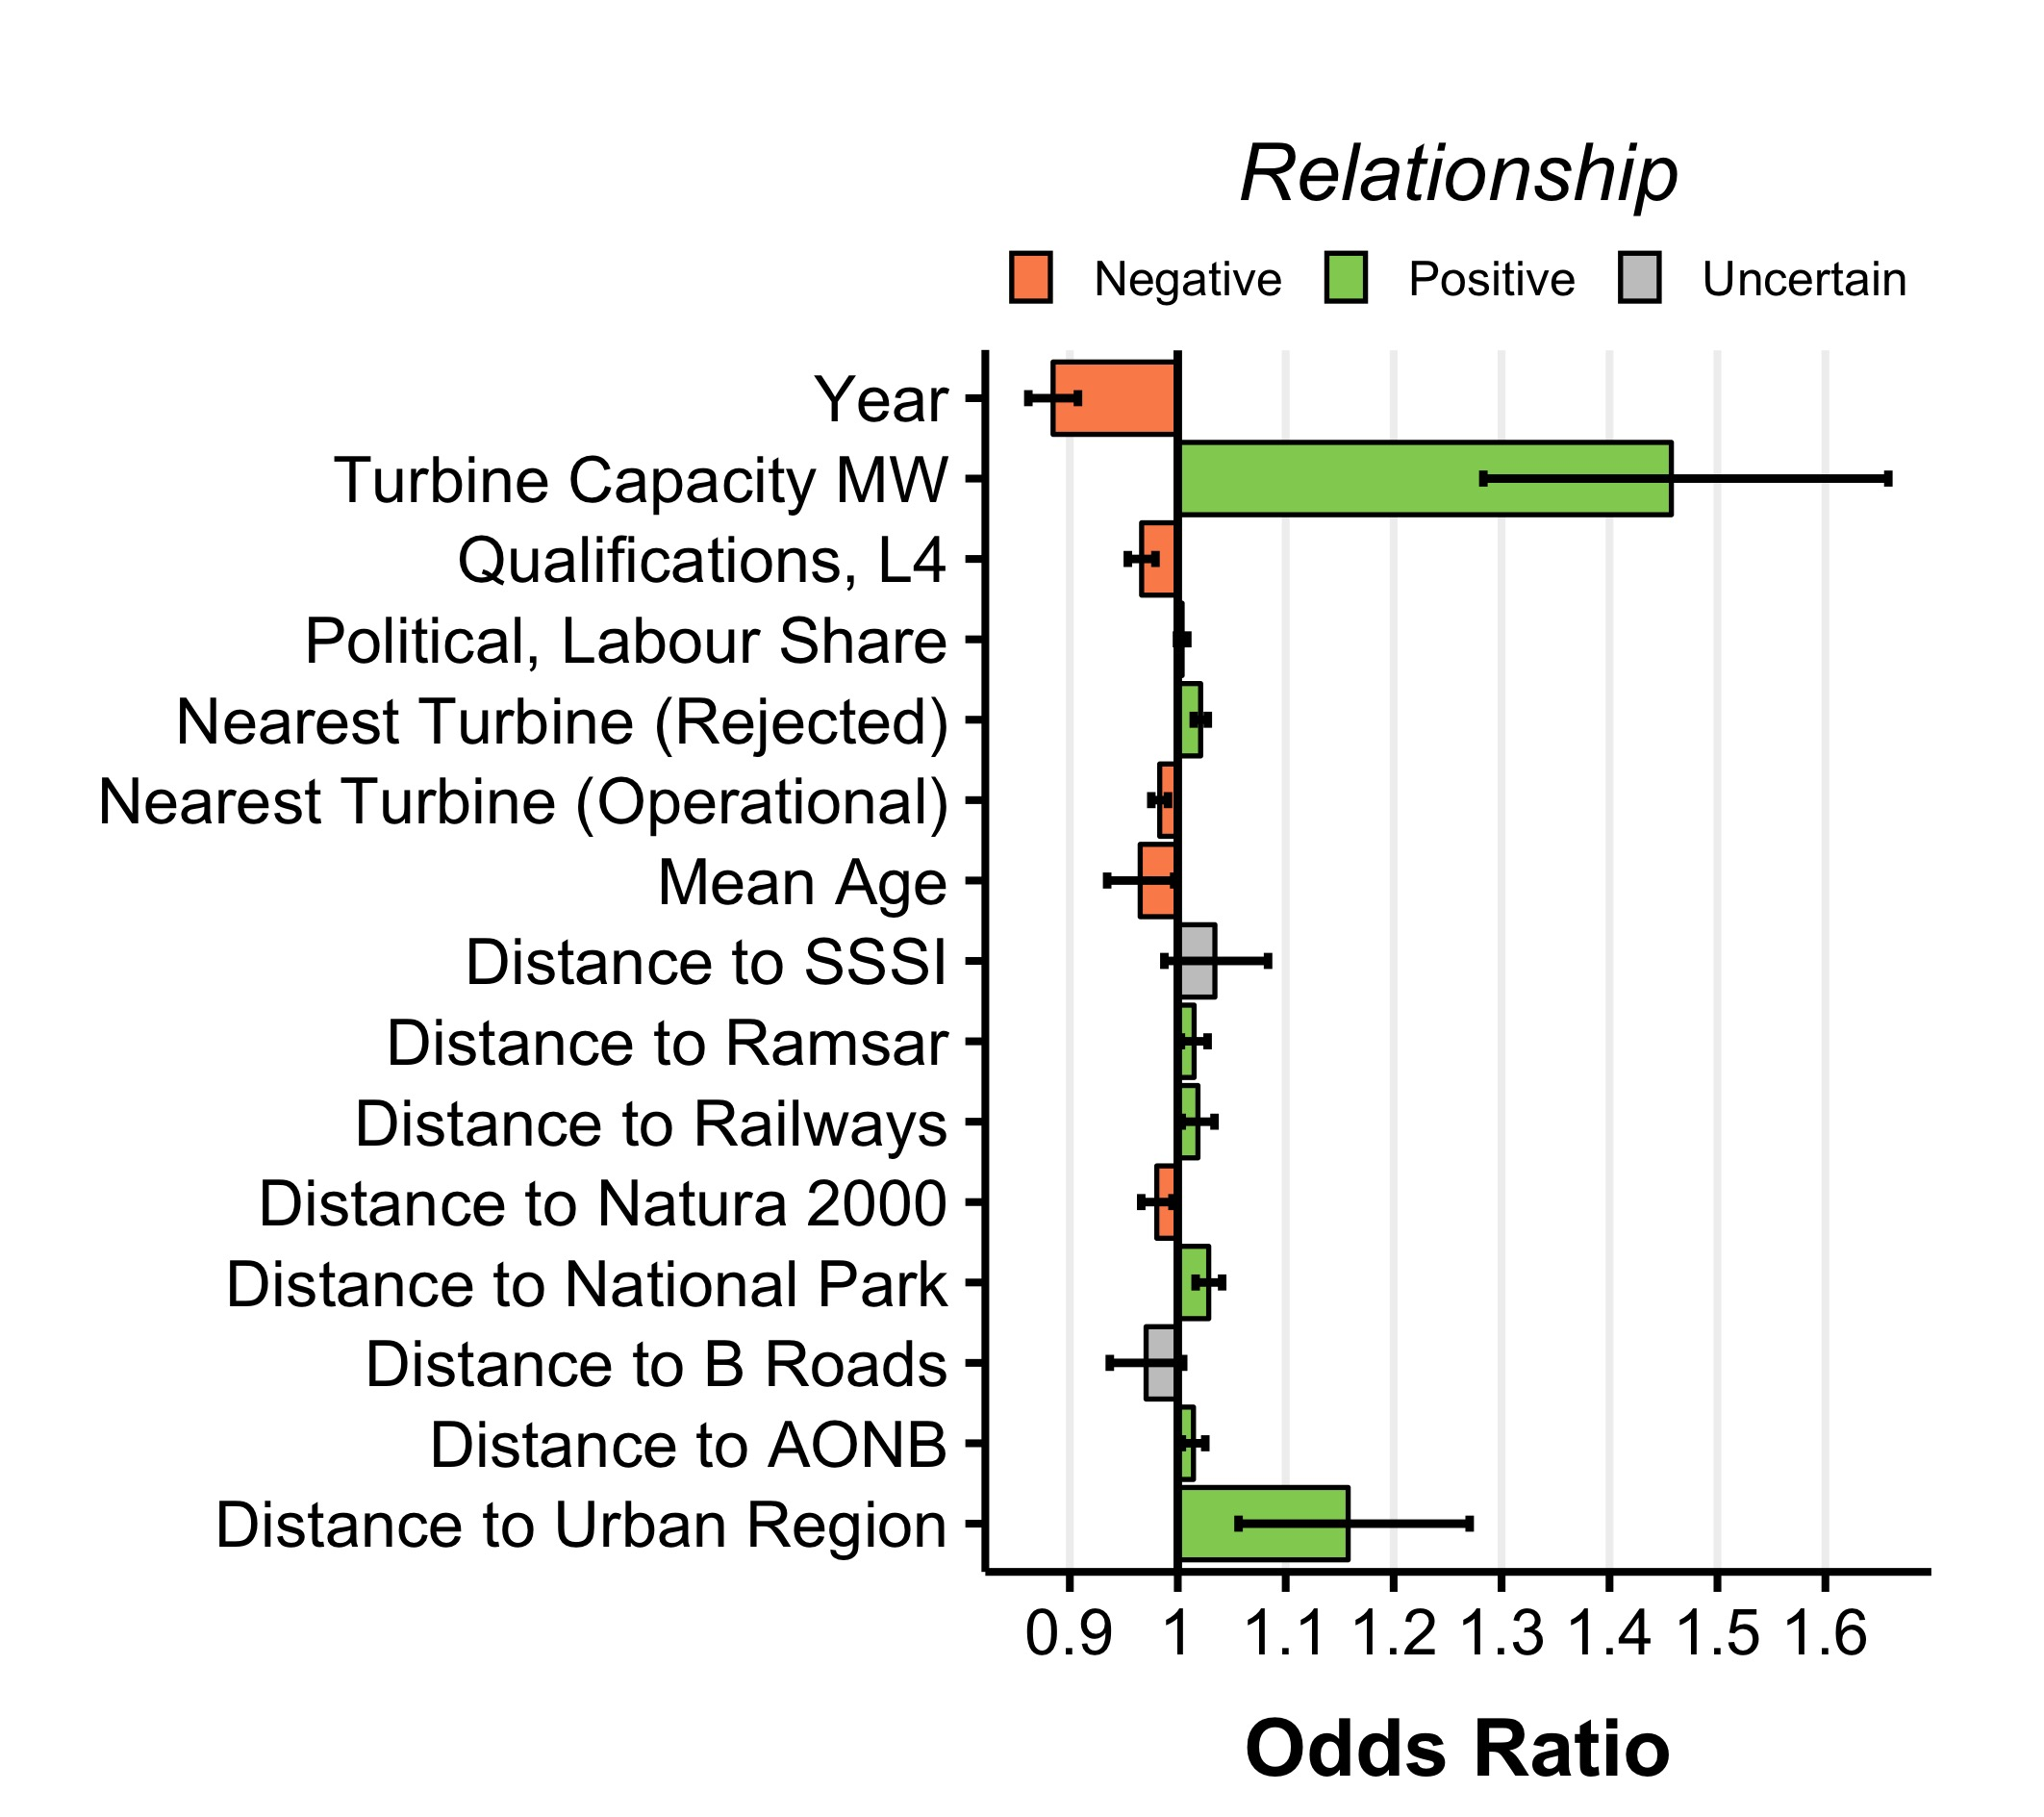
\includegraphics[width=0.5\linewidth]{figures/figure7} 

}

\caption{Odds Plot for Parsimonious Logistic Regression Model}\label{fig:oddsPars}
\end{figure}

The results of the nationally-segmented models are summarised in Table
\ref{tab:kableNestedModelResults}, comparing the \emph{Global
Parameters} against \emph{Optimised Parameters}. There has been a
general increase in the fit of the models represented by the Nagelkirke
R\textsuperscript{2} values. The difference between Odds Ratios between
each model is further highlighted in Table \ref{tab:segmented} for the
Global Parameters.

\begin{table}[!h]

\caption{\label{tab:kableNestedModelResults}Comparison of subset Logistic Regression Models based on the global parameters list}
\centering
\resizebox{\linewidth}{!}{
\begin{tabular}{llllllll}
\toprule
\multicolumn{2}{c}{ } & \multicolumn{3}{c}{Global Parameter} & \multicolumn{3}{c}{Optimised Parameters} \\
\cmidrule(l{2pt}r{2pt}){3-5} \cmidrule(l{2pt}r{2pt}){6-8}
  & Global & England & Scotland & Wales & England & Scotland & Wales\\
\midrule
Observations & 1715 & 772 & 787 & 156 & 772 & 787 & 156\\
Parameters & 16 & 16 & 16 & 16 & 10 & 13 & 9\\
Deviance & 2094 & 927 & 940 & 176 & 932 & 943 & 180\\
R.n & 0.198 & 0.209 & 0.232 & 0.302 & 0.202 & 0.228 & 0.275\\
Chi Square & 275 & 131 & 150 & 40 & 126 & 148 & 36\\
Degrees of Freedom & 15 & 15 & 15 & 15 & 9 & 12 & 8\\
p & 0.000 & 0.000 & 0.000 & 0.00045 & 0.000 & 0.000 & 2e-05\\
Residual Deviance & 1699 & 756 & 771 & 140 & 762 & 774 & 147\\
Accuracy & 66.6\% & 66.3\% & 67.4\% & 60.3\% & 67.5\% & 67.2\% & 63.6\%\\
\bottomrule
\end{tabular}}
\end{table}

\begin{table}[t]

\caption{\label{tab:segmented}Odds Ratios and significance for segmented regression models}
\centering
\begin{tabular}{lrlrlrl}
\toprule
\multicolumn{1}{c}{ } & \multicolumn{2}{c}{England} & \multicolumn{2}{c}{Scotland} & \multicolumn{2}{c}{Wales} \\
\cmidrule(l{2pt}r{2pt}){2-3} \cmidrule(l{2pt}r{2pt}){4-5} \cmidrule(l{2pt}r{2pt}){6-7}
Variable & OR &  & OR &  & OR & \\
\midrule
Turbine Capacity MW & 1.428 & *** & 1.562 & *** & 1.654 & *\\
Year & 0.882 & *** & 0.859 & *** & 0.919 & *\\
Distance to B Roads & 0.962 &  & 0.961 & . & 0.933 & \\
Distance to Railways & 0.987 &  & 1.027 & ** & 1.001 & \\
Distance to  Urban Region & 1.181 &  & 1.240 & *** & 1.158 & \\
Distance to AONB & 1.009 &  & 1.029 & ** & 1.083 & **\\
Distance to National Park & 1.032 & *** & 1.036 & ** & 1.073 & **\\
Distance to Ramsar & 1.012 &  & 1.030 & *** & 0.948 & \\
Distance to Natura 2000 & 0.986 &  & 0.970 & * & 0.916 & **\\
Distance to SSSI & 1.016 &  & 1.020 &  & 1.840 & ***\\
Qualifications, L4 & 0.969 & *** & 0.964 & ** & 0.984 & \\
Mean Age & 0.978 &  & 0.969 &  & 0.836 & .\\
Political, Labour Share & 1.005 &  & 0.996 &  & 1.014 & \\
Nearest Turbine (Operational) & 0.979 & *** & 0.987 & * & 0.991 & \\
Nearest Turbine (Rejected) & 1.024 & *** & 1.019 & *** & 1.012 & \\
\bottomrule
\multicolumn{7}{l}{\textit{Signif. codes:} 0 '***' 0.001 '**' 0.01 '*' 0.05 '.' 0.1 ' ' 1}\\
\end{tabular}
\end{table}

Finally, the results of the statistical generalisation are presented in
Figure \ref{fig:predictionRaster}, with sites being scored (0-100\%)
based on the predicted chance of project proposal. The average
acceptance value of the model is 21.9\%. Only 1.80\% of sites were
predicted to have a greater than 50\% chance of success, and 10.9\% of
sites were predicted to have an acceptance rate of less than 10\%.

\begin{figure}[h]

{\centering 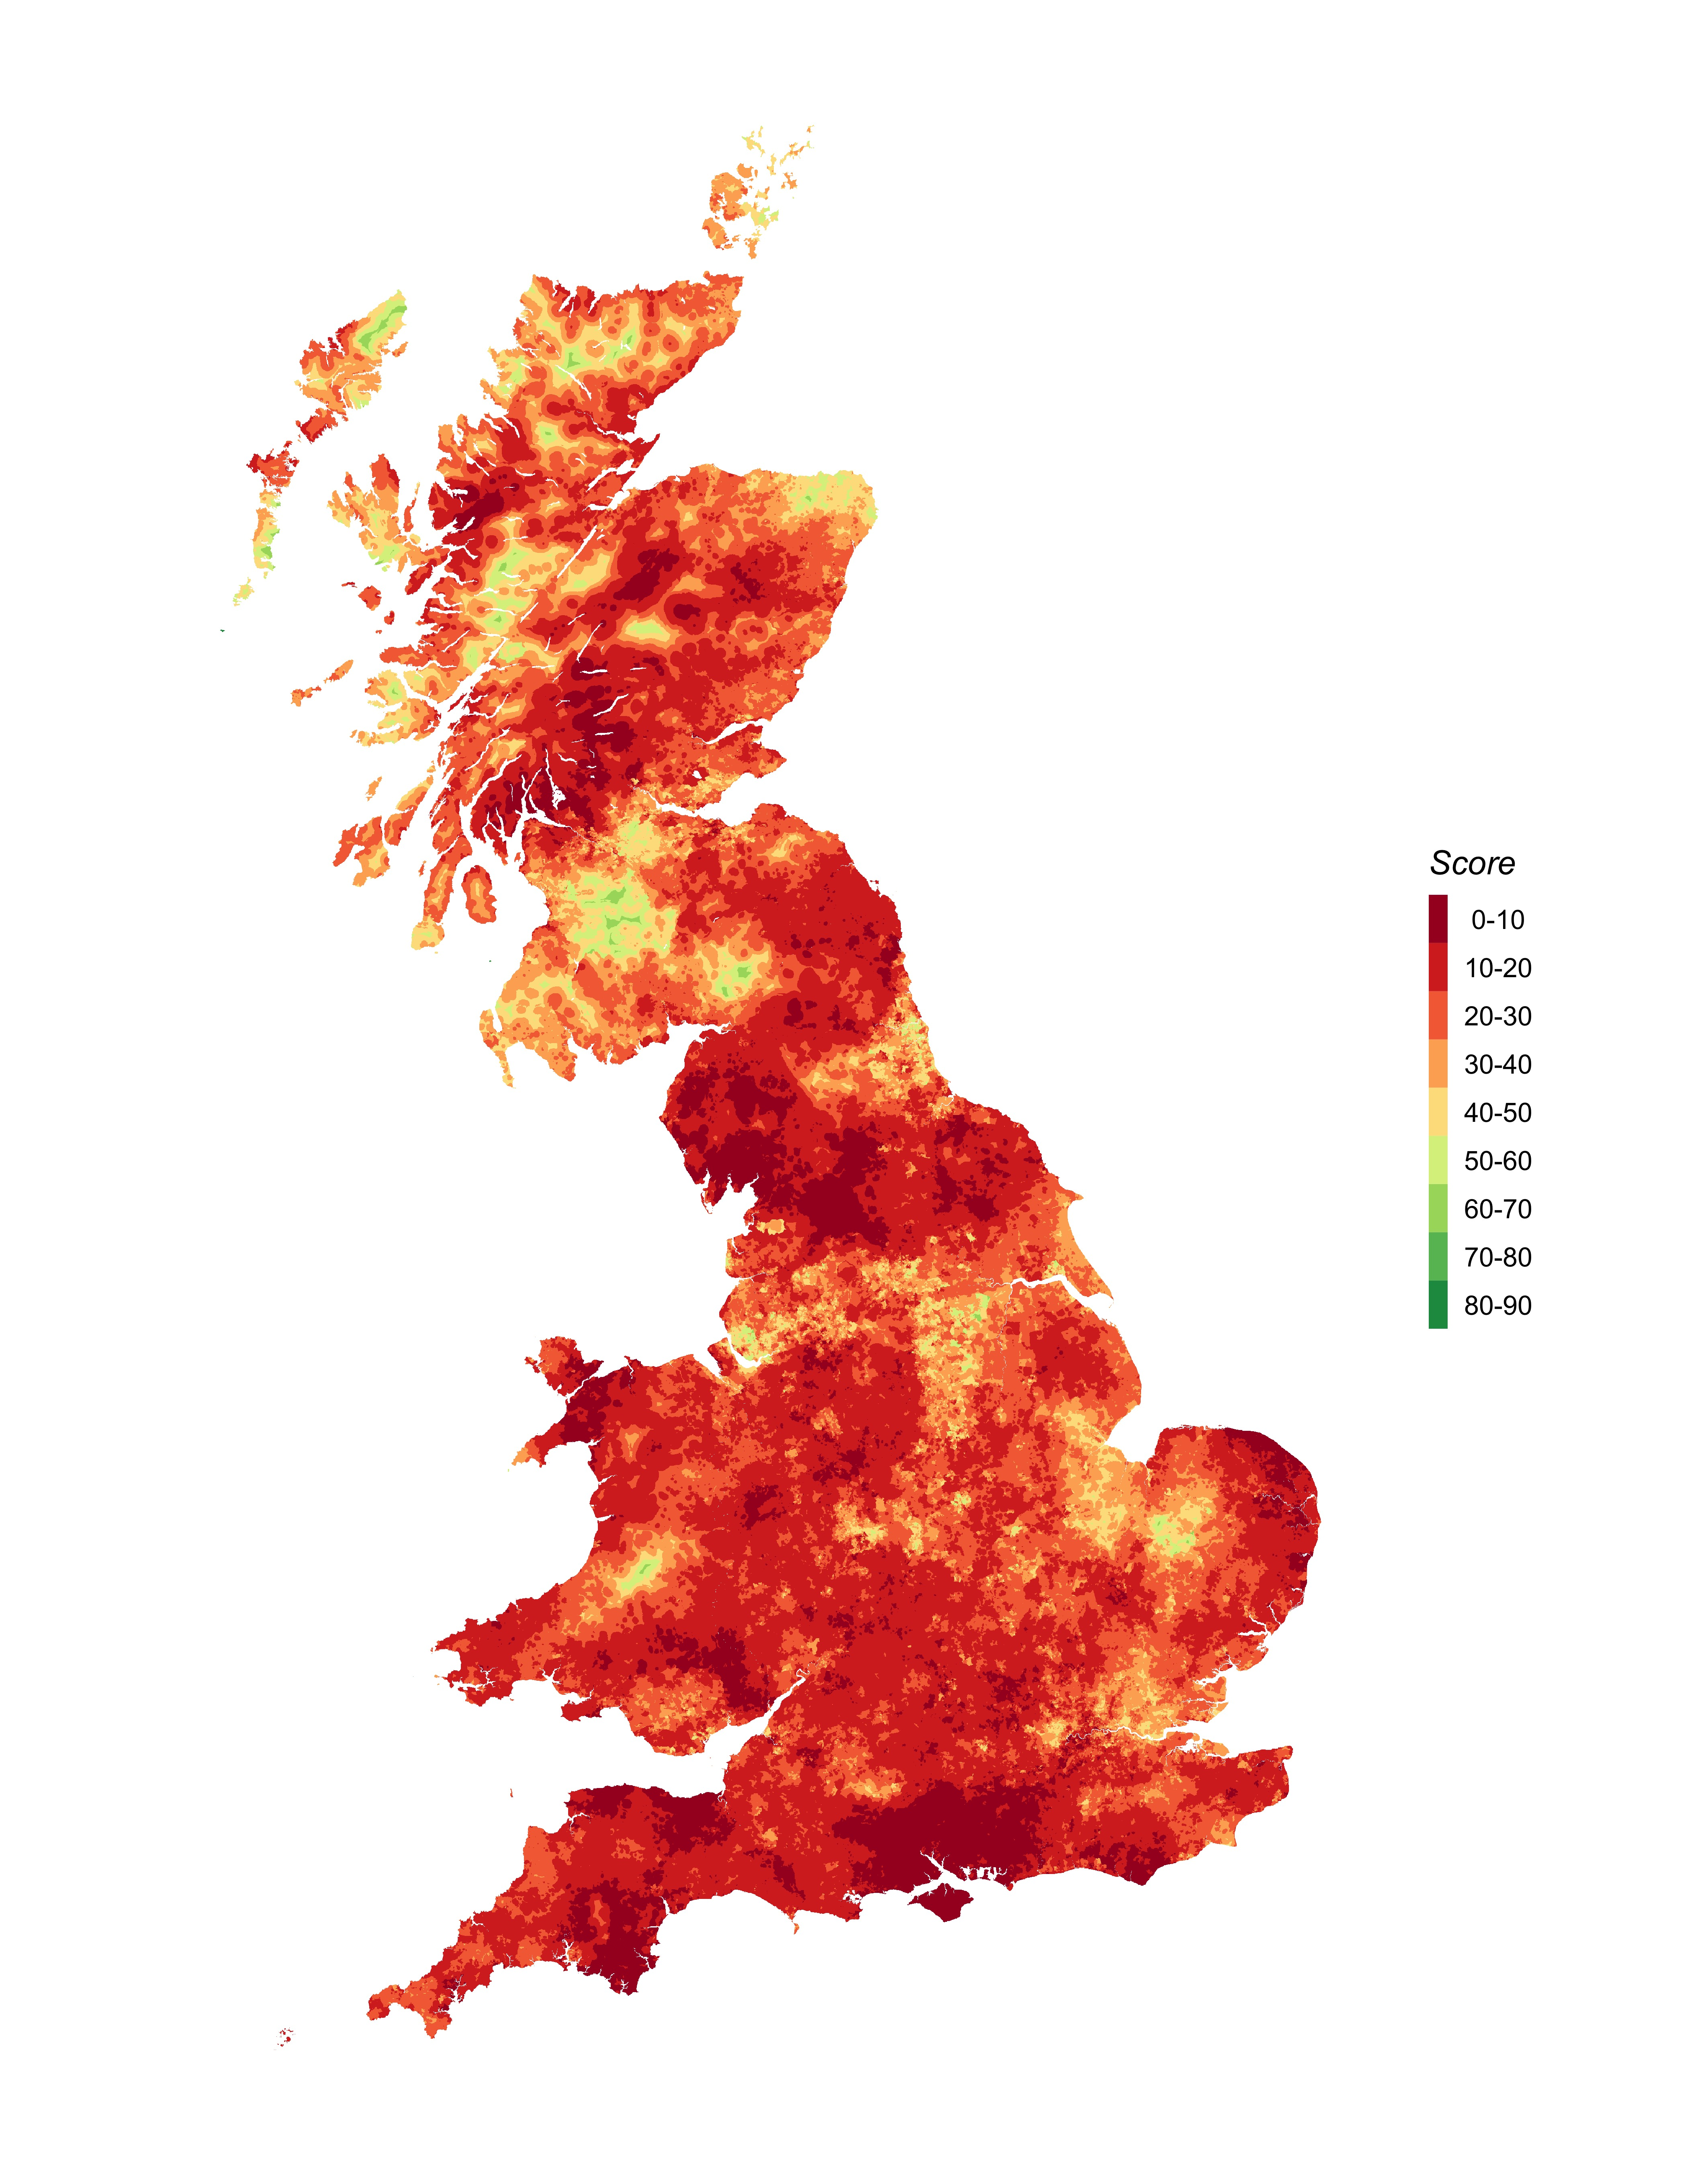
\includegraphics[width=1\linewidth]{figures/figure8} 

}

\caption{The generalised statistical model and predicted site acceptance for England, Scotland and Wales}\label{fig:predictionRaster}
\end{figure}

\hypertarget{discussion}{%
\section{Discussion}\label{discussion}}

\hypertarget{significant-parameters}{%
\subsection{Significant parameters}\label{significant-parameters}}

For project characteristics, the size of the turbine capacity is a
significant parameter, with larger turbines increasing the chance of
acceptance (note that this refers to the size of each individual
turbine, not the overall capacity of the project). This at first appears
counter intuitive, as it may be expected that smaller turbines cause a
lower visual impact and are therefore less opposed. However, there are
two options which are considered. Firstly, this result may suggest that
the developers of larger turbines are more likely to appeal the
decisions made against their projects, as rejection of such projects
would result in a large loss of potential revenue. Secondly, there is
evidence of correlation between turbine size and project (r = 0.35), and
that larger turbines are more likely to be in projects of over 50MW
which were previously influenced under the nationally significant
infrastructure, with such planning decisions potentially being more
favourable for projects as they reduce the local influence on projects.
However, it should be noted that this variable has a small standard
deviation (sd = 1.0) compared to other variables included within this
model, and therefore the non-standardised odds ratio inflates the
perceived influence of this variable.

The distance to urban areas was indicated to be statistically
significant, with sites further away from urban areas appearing more
socially acceptable, although there is considerable uncertainty as
indicated by the confidence interval. This supports the use of this
``classic'' parameter within existing geospatial models. There are a
number of potential causes for this: firstly, it could indicate that
high wind speed sites suitable for development tend to be naturally less
populated (i.e.~hilly, isolated regions). Additionally, it may reflect a
so-called ``Not in My Back Yard'' (NIMBY) view from the vocal local
population, with projects in closer proximity to urban areas being more
likely to be rejected. This has been a relatively contentious subject
within literature, with a range of studies supporting (Haggett and Toke
\protect\hyperlink{ref-Haggett2006}{2006}; Jones and Richard Eiser
\protect\hyperlink{ref-Jones2010}{2010}) and rejecting (Rensburg,
Kelley, and Jeserich \protect\hyperlink{ref-VanRensburg20}{2015};
Devine-Wright
\protect\hyperlink{ref-Devine-Wright2005a}{2005}\protect\hyperlink{ref-Devine-Wright2005a}{a};
Populus \protect\hyperlink{ref-Populus2005}{2005}) the NIMBY argument.
However this study provides quantitative evidence to suggest that sites
closer to urban areas have a lower chance of acceptance.

For landscape and environmental designations, distance to National
Parks, Ramsar and AONB were indicated as significant parameters, again
with sites being further away being suggested as more acceptable,
although these parameters have marginal impacts. This potentially
reflects the negative visual impacts which are often cited as a major
impact of wind energy developments (Langer et al.
\protect\hyperlink{ref-Langer2016}{2016}; Jones and Richard Eiser
\protect\hyperlink{ref-Jones2010}{2010}). However, it should be noted
that these influences have a relatively low impact, despite literature
indicating that landscape designations would play a more important role
(Langer et al. \protect\hyperlink{ref-Langer2016}{2016}).

The level of qualifications, and the mean age of the local population
have been retained as significant parameters for demographic variables.
Thus, the higher the proportion of people with higher qualifications and
the higher the local mean age, the less likely projects are to be
approved. This novel result suggests that regions of higher education
may be more effective in organising campaign groups against such
projects and supports the hypothesis developed by Van der Horst and Toke
(Horst and Toke \protect\hyperlink{ref-VanderHorst2010}{2010}) that
developers are likely to avoid more privileged areas. Conversely, there
are no statistically significant effects for share of local councillors
by political party, which suggests that individual political beliefs do
not influence the planning outcome of wind energy projects.

The analysis suggests that proximity to existing wind energy
developments may influence the likelihood of projects receiving
planning. The nearest operational wind energy project was indicated as
having a statistically significant effect, indicating that projects
further away from an existing project are less likely to be accepted. In
addition, the nearest rejected project is suggested to be have a
positive effect, inferring that the further the site is from a
previously rejected project, the higher the chance of acceptance. This
``proximity hypothesis'' has been a contentious subject challenged
within literature (Meyerhoff, Ohl, and Hartje
\protect\hyperlink{ref-Meyerhoff2010}{2010}; Ladenburg
\protect\hyperlink{ref-Ladenburg2008}{2008}; Eltham, Harrison, and Allen
\protect\hyperlink{ref-Eltham2008}{2008}) and this study provides
quantitative evidence to challenge this previous research.

There are notable parameters which are frequently used in GIS modelling,
but do not prove influential, including wind speed and the proximity to
airports. This may reflect that these parameters represent technical
challenges which can be investigated in the early stages of project
development, and therefore any sites that are not suitable will not
progress to seek planning permission.

It is interesting to note that despite including similar methodology as
the study by Roddis et al.~(\protect\hyperlink{ref-Roddis2018}{2018}),
there was limited overlap with the parameters used, with only 11 of the
30 parameters used in this study being shared between the two studies.
Of these parameters, supporting relationships were found between three
of these variables 1) \emph{Distance to National Parks} 2) \emph{Turbine
Capacity} and 3) \emph{Year of planning application}. However, as the
statistical model is not provided with the paper, it is not possible to
further assess the difference in greater detail, although there appear
to be opportunities to integrate the two methodologies proposed.

\hypertarget{model-fit}{%
\subsection{Model fit}\label{model-fit}}

The overall model fit of parameters is comparatively low based on
geospatial parameters alone, with the global parsimonious model
achieving a fit of 0.2. In comparison, the studies by Van Rensburg et
al.~(Rensburg, Kelley, and Jeserich
\protect\hyperlink{ref-VanRensburg20}{2015}) and Roddis et al (Roddis et
al. \protect\hyperlink{ref-Roddis2018}{2018}) achieved an overall
adjusted R\textsuperscript{2} value of 0.31 and 0.26 respectively.
Although fewer geospatial parameters were included within these studies,
they integrated greater number of institutional details and planning
details, which suggests that details of the planning process are a more
important indicator of site success than the spatial parameters alone.

\hypertarget{national-models}{%
\subsection{National models}\label{national-models}}

The split data model developed suggests that despite hypothesised
differences between the three nations, there is limited variation
between the significant influential parameters. Only \emph{Wind Speed}
exhibited variations in the positive and negative relationships, with
the model suggesting that sites in England have a greater chance of
acceptance at sites of higher windspeed whilst Wales and Scotland
reporting the opposite. However, the reduced number of observations used
to build each model increases the uncertainty substantially as indicated
by the greater confidence intervals.

\hypertarget{generalisation-1}{%
\subsection{Generalisation}\label{generalisation-1}}

The national prediction plot (Figure \ref{fig:predictionRaster}) shows
the estimated probability of success of wind turbines within Great
Britain. The results demonstrate that there are large regional
variations within wind energy site acceptability. For example, large
regions in Scotland appear suitable for development, while many other
regions and especially the South of England appear ``off limits'' to
development, particularly the regions along the South Coast of Great
Britain.

For the overall model, there is a low average predicted acceptance rate
of 21.9\% which is below the rate of acceptance of wind energy in Great
Britain, which was 40\% in 2017 (DECC
\protect\hyperlink{ref-DECC2018}{2018}). However, it would be expected
that the model would return a lower average, as sites which are selected
by developers will pass through several preselection criteria prior to
planning permission (Smith \protect\hyperlink{ref-Smith2016}{2016}).
Therefore, sites which are generally opposed before planning will often
be abandoned before being taken to planning permission.

The analysis results suggest that there is no ``one-size-fits-all''
approach for spatial modelling, and that there are large regional
variations in the development of wind energy projects beyond the
availability of the resource. In comparison, the regional renewable
energy studies conducted within Great Britain in 2010 broadly followed a
consistent methodology to assess the resource potential, with small
differences in the development rules in particular with regard to
environmental and landscape designations (Stoddart and Turley
\protect\hyperlink{ref-Stoddart2012}{2012}). In recent years, government
policy has shifted away from such top-down, standardised planning, and
it is therefore important that geospatial modelling aims to integrate
local context to more accurately capture this variation.

Surprisingly, the model suggests that the South West of England has a
low likelihood of acceptance, despite having high levels of wind energy
within the area. Great Britain's wind energy development largely started
in the region, so it had generally been considered supportive of wind
energy (Eltham, Harrison, and Allen
\protect\hyperlink{ref-Eltham2008}{2008}). Upon inspection, it can be
noted that this low level of acceptability is caused by the large number
of wind turbines and planning applications within the area, regional
demographics (high mean age) and proximity to protected landscapes.

Although the model makes spatial predictions for 2017, there are
difficulties forecasting beyond 2015 due to the changes within the
planning system explained within Section \ref{introduction}. These
changes granted greater control of onshore wind energy developments to
local communities, which has effectively allowed local communities to
block any wind energy developments. As the methodology does not
explicitly model planning constraints, it is not possible to assess this
shift in potential acceptance this has caused. However, there are
suggestions that the planning system may be reduce the difficulty in
constructing projects, and such a model may be able to more accurately
assess these changes. Therefore, the model results of this work can
provide a clear starting point for assessment of onshore UK wind if and
when local constraints are revised.

\hypertarget{conclusions-and-policy-recommendations}{%
\section{Conclusions and policy
recommendations}\label{conclusions-and-policy-recommendations}}

This paper has investigated the influence of geospatial, environmental,
demographic and political attributes on the probability of wind farm
planning approval in Great Britain between 1990 and 2015. The study
findings reveal that local demographic parameters are associated with
the planning outcomes of projects, and that many of the geospatial
parameters typically integrated into wind turbine models appear
insignificant in determining site approval.

The results raise concerns of the value of existing geospatial modelling
in assessing suitable locations for wind energy sites. These findings
provide evidence to support existing literature that such geospatial
tools in themselves are of limited applicability (Toke
\protect\hyperlink{ref-Toke2005}{2005}; Malczewski
\protect\hyperlink{ref-Malczewski2004}{2004}), and supports the
conclusion that greater emphasis needs to be given to the non-physical
elements of a project, such as local population attributes and potential
community engagement with the scheme from an early stage (Toke,
Breukers, and Wolsink \protect\hyperlink{ref-Toke2008}{2008}; Wolsink
\protect\hyperlink{ref-Wolsink2000}{2000}; Warren and McFadyen
\protect\hyperlink{ref-Warren2010}{2010}; Roddis et al.
\protect\hyperlink{ref-Roddis2018}{2018}). Other countries, most notably
Germany, place a much greater importance on ownership structures of
projects suggesting that locally owned projects may also be a much more
important factor than the geospatial parameters surrounding a site
(Warren and McFadyen \protect\hyperlink{ref-Warren2010}{2010}). These
findings therefore suggest that if a wind power developer can address
the oppositions from local residency, geospatial conditions will have
less influence to social acceptance.

Although the models have a relatively low overall fit, they are
consistent with previous research (Roddis et al.
\protect\hyperlink{ref-Roddis2018}{2018}; Rensburg, Kelley, and Jeserich
\protect\hyperlink{ref-VanRensburg20}{2015}), and there is value in the
generalisation of statistical model and resulting map of onshore wind
energy site suitability (Figure \ref{fig:predictionRaster}). With the
estimated cost of planning applications for commercial scale projects
exceeding £50,000 (Renewables First
\protect\hyperlink{ref-RF2016}{2016}), even marginal improvements in the
site selection process using these results could offer substantial cost
and risk reduction. This therefore allows a developer to filter out
areas which have positive geo-spatial conditions but more challenging
social acceptance conditions. This is the impact the study aims to bring
to the sector.

The findings from this model can help inform regional level energy
strategy by providing Local Authorities with the tools to understand
where and why developers may target turbine sites and the relative
importance of local physical, environmental and social attributes. Since
the modelling approach is repeatable it would also be possible to repeat
the model with additional locally relevant attributes and/or renewed
local demographic attributes to take account of local social change. The
results may also bring to the fore the possibility of an unintended
focusing of development on relatively disadvantaged areas through
developer targeting and/or local political decision-making processes.

The model raises important system implications within the UK's
electricity network. While there are specific regions which appear more
accepting of onshore wind, it may not be ideal for wind turbine
developments to be concentrated within these small areas. Such
concentration of wind development into small areas can result in grid
constraints and require additional capacity installed (Alexander, James,
and Richardson \protect\hyperlink{ref-alexander2014energy}{2014}) For
example, Dumfries and Galloway already suffers from major curtailment
issues due to lack of available grid capacity but is marked in places as
a likely site (DECC \protect\hyperlink{ref-DECC2016}{2016}). In
addition, focussing renewable energy resources into smaller regions can
reduce the security of supply of resources, as there is less
geographically dispersed variation in the resource (Engeland et al.
\protect\hyperlink{ref-ENGELAND2017600}{2017}). The results of this
analysis therefore require further detailed mapping for it to be used as
a decision-making tool.

The generalised model results highlight that there is large regional
variation within the site acceptability of onshore wind within Great
Britain. Regions of Scotland, England and Wales are suggested to be more
accepting of onshore wind projects, while there are large regions of low
acceptance notably the south-coast of England. Existing geospatial
modelling should integrate local understanding if they are to provide
realistic estimates of wind turbine sites, a finding which supports
existing literature (Langer et al.
\protect\hyperlink{ref-Langer2016}{2016}; Roddis et al.
\protect\hyperlink{ref-Roddis2018}{2018}), as ``\emph{traditional}'' GIS
which focusses on technical parameters may not capture the variation of
sites between regions.

As shown within the literature, studies have been conducted
internationally and have often reported conflicting issues surrounding
the social acceptance of projects (Scherhaufer et al.
\protect\hyperlink{ref-Scherhaufer2017}{2017}; Warren and McFadyen
\protect\hyperlink{ref-Warren2010}{2010}). As such, the results of this
study may therefore be specific to Great Britain. It is recommended that
international comparison is conducted using similar methods to provide
further insight into this potential national variation.

Great Britain provides an interesting international example in renewable
energy development, as energy policy has shifted towards a more hostile
stance against onshore wind energy since 2015. In particular, the
approval of planning has been granted to local communities, and it
appears that certain demographics are less accepting of onshore wind in
Great Britain. However, there are indications that legislation may be
altered to make wind turbine developments permitted in areas which are
generally supportive \emph{(Clean Growth Strategy/Outcomes of Bonn
COP23, HC596/597)}. The generalised map (Figure
\ref{fig:predictionRaster}) highlights that from a planning approval
rate, there are regions in the England and Wales which still appear
accepting of wind. As existing policy has effectively stalled onshore
wind within the country with the unintentional consequence to completely
block development, the results suggest that there would be opportunities
for future growth in onshore wind energy development in Great Britain.

\hypertarget{acknowledgments}{%
\subsection*{Acknowledgments}\label{acknowledgments}}
\addcontentsline{toc}{subsection}{Acknowledgments}

This work is part of the activities of the Energy and Climate Change
Division and the Sustainable Energy Research Group at the University of
Southampton \url{www.energy.soton.ac.uk}. It is also supported by ESPRC
under grant EP/J017698/1, Transforming the Engineering of Cities to
Deliver Societal and Planetary Wellbeing and the Faculty of Engineering
and Environment at the University of Southampton.

\hypertarget{reproducibility-statement}{%
\subsection*{Reproducibility
Statement}\label{reproducibility-statement}}
\addcontentsline{toc}{subsection}{Reproducibility Statement}

The data and supporting analysis are made available as supplementary
data for this. The analysis and report was written using the R
programming language and R Markdown (Allaire et al.
\protect\hyperlink{ref-R-rmarkdown}{2018}), with the full statistical
analysis and turbine dataset provided with the supporting files to allow
for the results of a the analysis to be reproduced.

\hypertarget{references}{%
\section*{References}\label{references}}
\addcontentsline{toc}{section}{References}

\let\oldhypertarget\hypertarget

\renewcommand{\hypertarget}[2]{%
    \leavevmode%
    \oldhypertarget{#1}{#2}%
}

\hypertarget{refs}{}
\leavevmode\hypertarget{ref-alexander2014energy}{}%
Alexander, Marcus Joseph, Patrick James, and Neil Richardson. 2014.
``Energy Storage Against Interconnection as a Balancing Mechanism for a
100\% Renewable Uk Electricity Grid.'' \emph{IET Renewable Power
Generation} 9 (2): 131--41.

\leavevmode\hypertarget{ref-R-rmarkdown}{}%
Allaire, JJ, Yihui Xie, Jonathan McPherson, Javier Luraschi, Kevin
Ushey, Aron Atkins, Hadley Wickham, Joe Cheng, and Winston Chang. 2018.
\emph{Rmarkdown: Dynamic Documents for R}.
\url{https://CRAN.R-project.org/package=rmarkdown}.

\leavevmode\hypertarget{ref-Atici2015}{}%
Atici, Kazim Baris, Ahmet Bahadir Simsek, Aydin Ulucan, and Mustafa Umur
Tosun. 2015. ``A GIS-based Multiple Criteria Decision Analysis approach
for wind power plant site selection.'' \emph{Utilities Policy} 37:
86--96. \url{https://doi.org/10.1016/j.jup.2015.06.001}.

\leavevmode\hypertarget{ref-Aydin2010}{}%
Aydin, Nazli Yonca, Elcin Kentel, and Sebnem Duzgun. 2010. ``GIS-based
environmental assessment of wind energy systems for spatial planning: A
case study from Western Turkey.'' \emph{Renewable and Sustainable Energy
Reviews} 14 (1): 364--73.
\url{https://doi.org/10.1016/j.rser.2009.07.023}.

\leavevmode\hypertarget{ref-Baban2001}{}%
Baban, Serwan M J, and Tim Parry. 2001. ``Developing and applying a
GIS-assisted approach to locating wind farms in the UK.''
\emph{Renewable Energy} 24 (1): 59--71.
\url{https://doi.org/10.1016/S0960-1481(00)00169-5}.

\leavevmode\hypertarget{ref-Baseer2017}{}%
Baseer, M.a., S. Rehman, J.P. Meyer, and Md. M. Alam. 2017. ``GIS-based
site suitability analysis for wind farm development in Saudi Arabia.''
\emph{Energy}. \url{https://doi.org/10.1016/j.energy.2017.10.016}.

\leavevmode\hypertarget{ref-Bright2006}{}%
Bright, J a, R H W Langston, R Bullman, R J Evans, S Gardner, J
Pearce-Higgins, and E Wilson. 2006. ``Bird sensitivity map to provide
locational guidance for onshore wind farms in Scotland'' 20 (20): i--ii,
1--136.
\href{\%3CGo\%20to\%20ISI\%3E://ZOOREC:ZOOR14403015814}{\textless{}Go to ISI\textgreater{}://ZOOREC:ZOOR14403015814}.

\leavevmode\hypertarget{ref-Brody2002}{}%
Brody, Julia Green, Donna J. Vorhees, Steven J. Melly, Susan R Swedis,
Peter Drivas, and Ruthann A. Rudel. 2002. ``Using Gis and Historical
Records to Reconstruct Residential Exposure to Large-Scale Pesticide
Application.'' \emph{Journal of Exposure Analysis and Environmental
Epidemiology} 12: 64--80.

\leavevmode\hypertarget{ref-Cirucci2014}{}%
Cirucci, John. 2014. ``Retrospective GIS-Based Multi-Criteria Decision
Analysis,'' no. December.

\leavevmode\hypertarget{ref-Cirucci2015}{}%
Cirucci, John F, Douglas A Miller, and Justine I Blanford. 2015.
``Retrospective GIS-Based Multi-Criteria Decision Analysis: A Case Study
of California Waste Transfer Station Siting Decisions.''
\emph{Proceedings of the International Symposium on Sustainable Systems
and Technologies} 3. \url{https://doi.org/10.6084/m9.figshare.1512514}.

\leavevmode\hypertarget{ref-Cowell2018}{}%
Cowell, Richard, and Patrick Devine-Wright. 2018. ``A
`delivery-democracy dilemma'? Mapping and explaining policy change for
public engagement with energy infrastructure.'' \emph{Journal of
Environmental Policy and Planning} 0 (0): 1--19.
\url{https://doi.org/10.1080/1523908X.2018.1443005}.

\leavevmode\hypertarget{ref-DECC2016}{}%
DECC. 2016. ``Renewable electricity in Scotland, Wales , Northern
Ireland and the regions of England in 2016.'' \emph{Energy Trends}.

\leavevmode\hypertarget{ref-DECC2018}{}%
---------. 2018. ``Renewable Energy Planning Database.''
\url{https://www.gov.uk/government/collections/renewable-energy-planning-data}.

\leavevmode\hypertarget{ref-DBIES2018}{}%
Department for Business Energy \& Industrial Strategy. 2018. ``Energy
and Climate Change Public Attitudes Tracker,'' no. April.

\leavevmode\hypertarget{ref-DBIES2016}{}%
Department for Business Energy \& Industry. 2016. ``Electricity
Generation Costs.''

\leavevmode\hypertarget{ref-Devine-Wright2005a}{}%
Devine-Wright, Patrick. 2005a. ``Beyond NIMBYism: Towards an integrated
framework for understanding public perceptions of wind energy.''
\emph{Wind Energy} 8 (2): 125--39. \url{https://doi.org/10.1002/we.124}.

\leavevmode\hypertarget{ref-Devine-Wright2005}{}%
---------. 2005b. ``Local aspects of UK renewable energy development:
exploring public beliefs and policy implications.'' \emph{Local
Environment} 10 (1): 57--69.
\url{https://doi.org/10.1080/1354983042000309315}.

\leavevmode\hypertarget{ref-Devine-Wright2007}{}%
---------. 2007. ``Reconsidering public attitudes and public acceptance
of renewable energy technologies : a critical review'' Working Paper.

\leavevmode\hypertarget{ref-DTI2001}{}%
DTI. 2001. ``NOABL Windspeed Database.'' \url{https://goo.gl/6BALyv}.

\leavevmode\hypertarget{ref-Eltham2008}{}%
Eltham, Douglas C., Gareth P. Harrison, and Simon J. Allen. 2008.
``Change in public attitudes towards a Cornish wind farm: Implications
for planning.'' \emph{Energy Policy} 36 (1): 23--33.
\url{https://doi.org/10.1016/j.enpol.2007.09.010}.

\leavevmode\hypertarget{ref-ENGELAND2017600}{}%
Engeland, Kolbjørn, Marco Borga, Jean-Dominique Creutin, Baptiste
François, Maria-Helena Ramos, and Jean-Philippe Vidal. 2017.
``Space-Time Variability of Climate Variables and Intermittent Renewable
Electricity Production -- a Review.'' \emph{Renewable and Sustainable
Energy Reviews} 79: 600--617.
\url{https://doi.org/https://doi.org/10.1016/j.rser.2017.05.046}.

\leavevmode\hypertarget{ref-Commission2015}{}%
European Commission. 2015. ``Digital Elevation Model over Europe
(EU-DEM).'' \url{http://www.eea.europa.eu/data-and-maps/data/eu-dem}.

\leavevmode\hypertarget{ref-EuropeanEnvironmentAgency2009}{}%
European Environment Agency. 2009. \emph{Europe's onshore and offshore
wind energy potential}. Vol. 6. 6. \url{https://doi.org/10.2800/11373}.

\leavevmode\hypertarget{ref-Fleming1979}{}%
Fleming, Michael D, and Roger M Hoffer. 1979. ``Machine Processing of
Landsat MSS Data and DMA Topographic Data for Forest Cover Type
Mapping.'' \emph{LARS Technical Report 082879 Laboratory for
Applications of Remote Sensing, Purdue University, West Lafayette,
Indiana.}, 377--90.

\leavevmode\hypertarget{ref-Garcia-Ayllon2013}{}%
Garcia-Ayllon, S. 2013. ``Retrospective analysis of urban development in
the Spanish Mediterranean coast.'' \emph{WIT Transactions on Ecology and
the Environment} 179 VOLUME (December 2013): 291--302.
\url{https://doi.org/10.2495/SC130251}.

\leavevmode\hypertarget{ref-Gass2013}{}%
Gass, Viktoria, Johannes Schmidt, Franziska Strauss, and Erwin Schmid.
2013. ``Assessing the economic wind power potential in Austria.''
\emph{Energy Policy} 53 (2013): 323--30.
\url{https://doi.org/10.1016/j.enpol.2012.10.079}.

\leavevmode\hypertarget{ref-Gigovic2017}{}%
Gigović, Ljubomir, Dragan Pamučar, Darko Božanić, and Srđan Ljubojević.
2017. ``Application of the GIS-DANP-MABAC multi-criteria model for
selecting the location of wind farms: A case study of Vojvodina,
Serbia.'' \emph{Renewable Energy} 103: 501--21.
\url{https://doi.org/10.1016/j.renene.2016.11.057}.

\leavevmode\hypertarget{ref-Gove2013}{}%
Gove, B, Rhw Langston, A McCluskie, Jd Pullan, and I Scrase. 2013.
``Wind farms and birds: an updated analysis of the effects of wind farms
on bird, and best practice guidance on integrated planning and impact
assessement.'' August.

\leavevmode\hypertarget{ref-Haggett2006}{}%
Haggett, Claire, and David Toke. 2006. ``Crossing the great divide-using
multi-method analysis to understand opposition to windfarms.''
\emph{Public Administration} 84 (1): 103--20.
\url{https://doi.org/10.1111/j.0033-3298.2006.00495.x}.

\leavevmode\hypertarget{ref-Hansen2005}{}%
Hansen, H. S. 2005. ``GIS-based Multi-Criteria Analysis of Wind Farm
Development.'' \emph{Proceedings of the 10th Scandinavian Research
Confrence on Geographical Information Scient}, 75--87.

\leavevmode\hypertarget{ref-Harper2018}{}%
Harper, Michael. 2018. ``Spatial planning scale for regional renewable
energy supply in the UK context.'' PhD thesis, University of
Southampton.

\leavevmode\hypertarget{ref-Harper2017}{}%
Harper, Michael, Ben Anderson, Patrick James, and A. S. Bahaj. 2017.
``Identifying key influences for planning acceptance of onshore wind
turbines.'' In \emph{Proceedings of Ecos 2017 - the 30th International
Conference on Efficiency, Cost, Optimization, Simulation and
Environmental Impact of Energy Systems}.

\leavevmode\hypertarget{ref-Harrell2001}{}%
Harrell, Frank E. 2001. \emph{Regression modeling strategies. With
applications to linear models, logistic regression, and survival
analysis}. \url{https://doi.org/10.1007/978-1-4757-3462-1}.

\leavevmode\hypertarget{ref-HMGovernment2014}{}%
HM Government. 2014. ``Planning Portal Northern Ireland.''

\leavevmode\hypertarget{ref-VanderHorst2010}{}%
Horst, Dan van der, and David Toke. 2010. ``Exploring the landscape of
wind farm developments; local area characteristics and planning process
outcomes in rural England.'' \emph{Land Use Policy} 27 (2): 214--21.
\url{https://doi.org/10.1016/j.landusepol.2009.05.006}.

\leavevmode\hypertarget{ref-Janke2010}{}%
Janke, J. R. 2010. ``Multicriteria GIS modeling of wind and solar farms
in Colorado.'' \emph{Renewable Energy} 35: 2228--34.

\leavevmode\hypertarget{ref-Jones2011}{}%
Jones, Christopher R., Barry J. Orr, and J. Richard Eiser. 2011. ``When
is enough, enough? Identifying predictors of capacity estimates for
onshore wind-power development in a region of the UK.'' \emph{Energy
Policy} 39 (8): 4563--77.
\url{https://doi.org/10.1016/j.enpol.2011.04.044}.

\leavevmode\hypertarget{ref-Jones2010}{}%
Jones, Christopher R., and J. Richard Eiser. 2010. ``Understanding
'local' opposition to wind development in the UK: How big is a
backyard?'' \emph{Energy Policy} 38 (6): 3106--17.
\url{https://doi.org/10.1016/j.enpol.2010.01.051}.

\leavevmode\hypertarget{ref-Kazak2017}{}%
Kazak, Jan, Joost van Hoof, and Szymon Szewranski. 2017. ``Challenges in
the wind turbines location process in Central Europe -- The use of
spatial decision support systems.'' \emph{Renewable and Sustainable
Energy Reviews} 76 (February): 425--33.
\url{https://doi.org/10.1016/j.rser.2017.03.039}.

\leavevmode\hypertarget{ref-Krohn1999}{}%
Krohn, Soren, and Steffen Damborg. 1999. ``On Public Attitudes Towards
Wind Power.'' \emph{Renewable Energy} 16: 954--60.
\url{https://doi.org/10.1016/S0960-1481(98)00339-5}.

\leavevmode\hypertarget{ref-Ladenburg2008}{}%
Ladenburg, Jacob. 2008. ``Attitudes towards on-land and offshore wind
power development in Denmark; choice of development strategy.''
\emph{Renewable Energy} 33 (1): 111--18.
\url{https://doi.org/10.1016/j.renene.2007.01.011}.

\leavevmode\hypertarget{ref-Langer2016}{}%
Langer, Katharina, Thomas Decker, Jutta Roosen, and Klaus Menrad. 2016.
``A qualitative analysis to understand the acceptance of wind energy in
Bavaria.'' \emph{Renewable and Sustainable Energy Reviews} 64: 248--59.
\url{https://doi.org/10.1016/j.rser.2016.05.084}.

\leavevmode\hypertarget{ref-Lee2009}{}%
Lee, Amy H I, Hsing Hung Chen, and He Yau Kang. 2009. ``Multi-criteria
decision making on strategic selection of wind farms.'' \emph{Renewable
Energy} 34 (1): 120--26.
\url{https://doi.org/10.1016/j.renene.2008.04.013}.

\leavevmode\hypertarget{ref-Liu2017}{}%
Liu, Changyi, Yang Wang, and Rong Zhu. 2017. ``Assessment of the
economic potential of China's onshore wind electricity.''
\emph{Resources, Conservation and Recycling} 121: 33--39.
\url{https://doi.org/10.1016/j.resconrec.2016.10.001}.

\leavevmode\hypertarget{ref-Malczewski2004}{}%
Malczewski, Jacek. 2004. ``GIS-based land-use suitability analysis: A
critical overview.'' \emph{Progress in Planning} 62 (1): 3--65.
\url{https://doi.org/10.1016/j.progress.2003.09.002}.

\leavevmode\hypertarget{ref-Manomaiphiboon2017}{}%
Manomaiphiboon, Kasemsan, Carina P. Paton, Thayukorn Prabamroong, Nuttee
Rajpreeja, Nosha Assareh, and Montana Siriwan. 2017. ``Wind energy
potential analysis for Thailand: Uncertainty from wind maps and
sensitivity to turbine technology.'' \emph{International Journal of
Green Energy} 14 (6): 528--39.
\url{https://doi.org/10.1080/15435075.2017.1305963}.

\leavevmode\hypertarget{ref-Mentis2017}{}%
Mentis, Dimitris, Shahid Hussain Siyal, Alexandros Korkovelos, and Mark
Howells. 2017. ``Estimating the spatially explicit wind generated
electricity cost in Africa - A GIS based analysis.'' \emph{Energy
Strategy Reviews} 17: 45--49.
\url{https://doi.org/10.1016/j.esr.2017.07.002}.

\leavevmode\hypertarget{ref-Meyerhoff2010}{}%
Meyerhoff, Jurgen, Cornelia Ohl, and Volkmar Hartje. 2010. ``Landscape
externalities from onshore wind power.'' \emph{Energy Policy} 38 (1):
82--92. \url{https://doi.org/10.1016/j.enpol.2009.08.055}.

\leavevmode\hypertarget{ref-Miller2014}{}%
Miller, Adam, and Ruopu Li. 2014. ``A Geospatial Approach for
Prioritizing Wind Farm Development in Northeast Nebraska, USA.''
\emph{ISPRS International Journal of Geo-Information} 3 (3): 968--79.
\url{https://doi.org/10.3390/ijgi3030968}.

\leavevmode\hypertarget{ref-Mohamed2004}{}%
Mohamed, Noha Saleh, Laila Mohamed Nofal, Mona Hassan Ahmed Hassan, and
Saleh Mesbah Elkaffas. 2004. ``Geographic information systems (GIS)
analysis of under five mortality in Alexandria.'' \emph{The Journal of
the Egyptian Public Health Association} 79 (3-4): 243--62.

\leavevmode\hypertarget{ref-Neufville2013}{}%
Neufville, Laurence. 2013. ``Wind farm Site Suitability Selection using
Multi-Criteria Analysis (MCA) and Spatial Modelling,'' no. July: 1--29.

\leavevmode\hypertarget{ref-Noorollahi2015}{}%
Noorollahi, Younes, Hossein Yousefi, and Mohammad Mohammadi. 2015.
``Multi-criteria decision support system for wind farm site selection
using GIS.'' \emph{Sustainable Energy Technologies and Assessments} 13:
38--50. \url{https://doi.org/10.1016/j.seta.2015.11.007}.

\leavevmode\hypertarget{ref-OfficeforNationalStatistics}{}%
Office for National Statistics. 2016. ``2011 Census data.''
\url{https://www.ons.gov.uk/census/2011census/2011censusdata}.

\leavevmode\hypertarget{ref-ONS2013}{}%
ONS. 2013. ``2011 Census, Quick Statistics for Wales on National
Identity, Passports Held and Country of Birth.''

\leavevmode\hypertarget{ref-Survey2016}{}%
Ordnance Survey. 2016. ``OS Strategi.''
\url{https://data.gov.uk/dataset/strategi}.

\leavevmode\hypertarget{ref-Overpass2016}{}%
OSM. 2016. ``Overpass API.'' \url{https://overpass-turbo.eu/}.

\leavevmode\hypertarget{ref-Pope2017}{}%
Pope, Addy. 2017. ``UK National Parks.''
\url{http://dx.doi.org/10.7488/ds/1810}.

\leavevmode\hypertarget{ref-Populus2005}{}%
Populus. 2005. ``Energy Balance of Power Poll Fieldwork : July 1st-6th
2005,'' 1--23.

\leavevmode\hypertarget{ref-R-base}{}%
R Core Team. 2018. \emph{R: A Language and Environment for Statistical
Computing}. Vienna, Austria: R Foundation for Statistical Computing.
\url{https://www.R-project.org/}.

\leavevmode\hypertarget{ref-RF2016}{}%
Renewables First. 2016. ``Wind Turbine Planning Permission.''
\url{http://www.renewablesfirst.co.uk/windpower/wind-turbine-consenting/wind-turbine-planning-permission/}.

\leavevmode\hypertarget{ref-VanRensburg20}{}%
Rensburg, Thomas M. van, Hugh Kelley, and Nadine Jeserich. 2015. ``What
influences the probability of wind farm planning approval: Evidence from
Ireland.'' \emph{Ecological Economics} 111: 12--22.
\url{https://doi.org/10.1016/j.ecolecon.2014.12.012}.

\leavevmode\hypertarget{ref-Roddis2018}{}%
Roddis, Philippa, Stephen Carver, Martin Dallimer, Paul Norman, and Guy
Ziv. 2018. ``The role of community acceptance in planning outcomes for
onshore wind and solar farms : An energy justice analysis.''
\emph{Applied Energy} 226 (October 2017): 353--64.
\url{https://doi.org/10.1016/j.apenergy.2018.05.087}.

\leavevmode\hypertarget{ref-Scherhaufer2017}{}%
Scherhaufer, Patrick, Stefan Höltinger, Boris Salak, Thomas
Schauppenlehner, and Johannes Schmidt. 2017. ``Patterns of acceptance
and non-acceptance within energy landscapes: Acase study on wind energy
expansion in Austria.'' \emph{Energy Policy} 109 (May): 863--70.
\url{http://dx.doi.org/10.1016/j.enpol.2017.05.057}.

\leavevmode\hypertarget{ref-Sliz-Szkliniarz2011}{}%
Sliz-Szkliniarz, Beata, and Joachim Vogt. 2011. \emph{Renewable and
Sustainable Energy Reviews} 15 (3): 1696--1707.

\leavevmode\hypertarget{ref-Smith2016}{}%
Smith, Louise. 2016. ``Planning for onshore wind farms.'' \emph{House of
Commons Briefing Paper}, no. 04370.
\url{http://www.parliament.uk/briefing-papers/sn04370.pdf}.

\leavevmode\hypertarget{ref-SNH2009}{}%
SNH. 2009. ``Siting and Designing windfarms in the landscape,'' no.
December.

\leavevmode\hypertarget{ref-Sonnberger2017}{}%
Sonnberger, Marco, and Michael Ruddat. 2017. ``Local and socio-political
acceptance of wind farms in Germany.'' \emph{Technology in Society} 51:
56--65. \url{http://dx.doi.org/10.1016/j.techsoc.2017.07.005}.

\leavevmode\hypertarget{ref-SQWEnergy2010}{}%
SQW Energy. 2010. ``Renewable and Low-carbon Energy Capacity Methodology
Methodology for the English Regions.'' January.

\leavevmode\hypertarget{ref-Stoddart2012}{}%
Stoddart, Harley, and David Turley. 2012. ``Review of approaches adopted
in regional renewable energy capacity assessments when following the
Regional Renewable and Low Carbon Energy Capacity Methodology.'' June.

\leavevmode\hypertarget{ref-Stoltzfus2011}{}%
Stoltzfus, Jill C. 2011. ``Logistic regression: A brief primer.''
\emph{Academic Emergency Medicine} 18 (10): 1099--1104.
\url{https://doi.org/10.1111/j.1553-2712.2011.01185.x}.

\leavevmode\hypertarget{ref-Strachan2004}{}%
Strachan, Peter a., and David Lal. 2004. ``Wind energy policy, planning
and management practice in the UK: Hot air or a gathering storm?''
\emph{Regional Studies} 38 (5): 551--71.
\url{https://doi.org/10.1080/0143116042000229311}.

\leavevmode\hypertarget{ref-Toke2005}{}%
Toke, Dave. 2005. ``Explaining wind power planning outcomes: Some
findings from a study in England and Wales.'' \emph{Energy Policy} 33
(12): 1527--39. \url{https://doi.org/10.1016/j.enpol.2004.01.009}.

\leavevmode\hypertarget{ref-Toke2008}{}%
Toke, David, Sylvia Breukers, and Maarten Wolsink. 2008. ``Wind power
deployment outcomes: How can we account for the differences?''
\emph{Renewable and Sustainable Energy Reviews} 12 (4): 1129--47.
\url{https://doi.org/10.1016/j.rser.2006.10.021}.

\leavevmode\hypertarget{ref-UNEP2016}{}%
UNEP. 2016. ``Global trends in renewable energy.''

\leavevmode\hypertarget{ref-Upham2015}{}%
Upham, Paul, Christian Oltra, and Àlex Boso. 2015. ``Towards a
cross-paradigmatic framework of the social acceptance of energy
systems.'' \emph{Energy Research \& Social Science} 8: 100--112.
\url{https://doi.org/10.1016/j.erss.2015.05.003}.

\leavevmode\hypertarget{ref-USEPA2002}{}%
US EPA, OSWER Office of Resource Conservation, and Recovery. 2002.
``Waste Transfer Stations: A Manual for Decision-Making,'' 1--66.
\url{papers3://publication/uuid/7CAEDFA2-1B14-4CFF-8B13-1E920D35AD80}.

\leavevmode\hypertarget{ref-VanHaaren2011}{}%
Van Haaren, Rob, and Vasilis Fthenakis. 2011. ``GIS-based wind farm site
selection using spatial multi-criteria analysis (SMCA): Evaluating the
case for New York State.'' \emph{Renewable and Sustainable Energy
Reviews} 15 (7): 3332--40.
\url{https://doi.org/10.1016/j.rser.2011.04.010}.

\leavevmode\hypertarget{ref-Voivontas1998}{}%
Voivontas, D., D. Assimacopoulos, a. Mourelatos, and J. Corominas. 1998.
``Evaluation of renewable energy potential using a GIS decision support
system.'' \emph{Renewable Energy} 13 (3): 333--44.
\url{https://doi.org/10.1016/S0960-1481(98)00006-8}.

\leavevmode\hypertarget{ref-Wang2014}{}%
Wang, Qianna, Martin Mwirigi M'Ikiugu, and Isami Kinoshita. 2014. ``A
GIS-based approach in support of spatial planning for renewable energy:
A case study of Fukushima, Japan.'' \emph{Sustainability (Switzerland)}
6 (4): 2087--2117. \url{https://doi.org/10.3390/su6042087}.

\leavevmode\hypertarget{ref-Warren2005}{}%
Warren, Charles R., Carolyn Lumsden, Simone O'Dowd, and Richard V.
Birnie. 2005. ``'Green On Green': Public perceptions of wind power in
Scotland and Ireland.'' \emph{Journal of Environmental Planning and
Management} 48 (July): 853--75.
\url{https://doi.org/10.1080/09640560500294376}.

\leavevmode\hypertarget{ref-Warren2010}{}%
Warren, Charles R., and Malcolm McFadyen. 2010. ``Does community
ownership affect public attitudes to wind energy? A case study from
south-west Scotland.'' \emph{Land Use Policy} 27 (2): 204--13.
\url{https://doi.org/10.1016/j.landusepol.2008.12.010}.

\leavevmode\hypertarget{ref-Watson2015}{}%
Watson, Joss J W, and Malcolm D. Hudson. 2015. ``Regional Scale wind
farm and solar farm suitability assessment using GIS-assisted
multi-criteria evaluation.'' \emph{Landscape and Urban Planning} 138:
20--31. \url{https://doi.org/10.1016/j.landurbplan.2015.02.001}.

\leavevmode\hypertarget{ref-Wolsink2000}{}%
Wolsink, Maarten. 2000. ``Wind power and the NIMBY-myth: institutional
capacity and the limited significance of public support.''
\emph{Renewable Energy} 21 (1): 49--64.
\url{https://doi.org/10.1016/S0960-1481(99)00130-5}.

\leavevmode\hypertarget{ref-Wustenhagen2007}{}%
Wustenhagen, Rolf, Maarten Wolsink, and Mary Jean Burer. 2007. ``Social
acceptance of renewable energy innovation: An introduction to the
concept.'' \emph{Energy Policy} 35 (5): 2683--91.
\url{https://doi.org/10.1016/j.enpol.2006.12.001}.

\leavevmode\hypertarget{ref-Yamada2009}{}%
Yamada, Ikuho, Peter A. Rogerson, and Gyoungju Lee. 2009.
``GeoSurveillance: A GIS-based system for the detection and monitoring
of spatial clusters.'' \emph{Journal of Geographical Systems} 11 (2):
155--73.

\leavevmode\hypertarget{ref-Yue2006}{}%
Yue, Cheng D., and Shi Sian Wang. 2006. ``GIS-based evaluation of
multifarious local renewable energy sources: A case study of the Chigu
area of southwestern Taiwan.'' \emph{Energy Policy} 34 (6): 730--42.
\url{https://doi.org/10.1016/j.enpol.2004.07.003}.

\newpage

\begin{landscape}\begin{table}[t]

\caption{\label{tab:unnamed-chunk-3}Summary of data sources used within model}
\centering
\resizebox{\linewidth}{!}{
\begin{tabular}{rlllllll}
\toprule
ID & Category & Variable & Source & Data Type & Variable Value & Value Type & Unit\\
\midrule
1 & Turbine & Wind Turbine Planning Data & REPD (DECC, 2016) & Tabular & Planning Outcome & Categorical & Accept/Reject\\
2 &  & Turbine Capacity &  & Tabular & Megawatts/turbine & Continuous & MW\\
3 &  & Number of Turbines &  & Tabular &  & Continuous & \\
4 &  & Year &  & Tabular &  & Discrete & \\
5 &  & Country &  & Tabular &  & Categorical & \\
6 & Resource & Wind Speed & NOABL (DTI, 2001) & Raster & Annualised Wind Speed & Continuous & m/s\\
7 & Features & Airports & OpenGeo & Points & Distance to Feature & Continuous & km\\
8 &  & Roads\textsuperscript{a} & OS Strategi (Ordnance Survey, 2016) & Lines & Distance to Feature & Continuous & km\\
9 &  & Railways &  & Lines & Distance to Feature & Continuous & km\\
10 &  & Urban Areas &  & Polygons & Distance to Feature & Continuous & km\\
11 &  & HV Powerlines\textsuperscript{b} & OSM & Lines & Distance to Feature & Continuous & km\\
12 &  & Military Sites & OSM & Points, Polygons & Distance to Feature & Continuous & km\\
13 & Landscape & Areas of Outstanding Natural Beauty & National Heritage & Polygons & Distance to Feature & Continuous & km\\
14 &  & National Parks &  & Polygons & Distance to Feature & Continuous & km\\
15 &  & Heritage Coast &  & Polygons & Distance to Feature & Continuous & km\\
16 & Nature & Special Protection Areas &  & Polygons & Distance to Feature & Continuous & km\\
17 &  & National Nature Reserve &  & Polygons & Distance to Feature & Continuous & km\\
18 &  & Sites of Special Scientific Interest &  & Polygons & Distance to Feature & Continuous & km\\
19 &  & Special Areas of Conservation &  & Polygons & Distance to Feature & Continuous & km\\
20 & Geographic & Elevation & EU DEM & Raster & Height above sea level & Integer & m\\
21 &  & Slope & Derived from 18 & Raster & Gradient & Continuous & \%\\
22 & Census & Level of Qualification\textsuperscript{c} & ONS & Tabular & Higher than L4 & Continuous & \%\\
23 &  & Age &  & Tabular & Mean & Continuous & Years\\
24 &  & Social Grade\textsuperscript{d} &  & Tabular & Social Grade AB & Continuous & \%\\
25 &  & Tenure &  & Tabular & Home Ownership & Continuous & \%\\
26 & Political & Conservatives & Populus & Tabular & Percentage of Council & Continuous & \%\\
27 &  & Labour &  & Tabular & Percentage of Council & Continuous & \%\\
28 &  & Liberal Democrat &  & Tabular & Percentage of Council & Continuous & \%\\
29 & Proximity & Nearest Turbine (Operational) & Calculated & Points & Distance to Turbine & Continuous & km\\
30 &  & Nearest Turbine (Rejected) & Calculated & Points & Distance to Turbine & Continuous & km\\
\bottomrule
\multicolumn{8}{l}{\textsuperscript{a} Roads are broken into four main categories: Motorways, A Roads, B Roads and Minor Roads}\\
\multicolumn{8}{l}{\textsuperscript{b} High Voltage network from 132 kV to 400 kV}\\
\multicolumn{8}{l}{\textsuperscript{c} L4 represents degree level or above}\\
\multicolumn{8}{l}{\textsuperscript{d} AB represents Higher and intermediate managerial, administrative, professional occupation}\\
\end{tabular}}
\end{table}
\end{landscape}


\end{document}
